\documentclass[numbers=noenddot, 12pt, a4paper, oneside]{scrbook}
\usepackage{blindtext}
\usepackage[utf8]{inputenc}
\usepackage{subcaption}
\usepackage{float}
\usepackage{tabularx}
\usepackage{graphicx}
\def\Plus{\texttt{+}}
\usepackage{listings}
\usepackage{color}
\usepackage{dirtytalk}

\definecolor{dkgreen}{rgb}{0,0.6,0}
\definecolor{gray}{rgb}{0.5,0.5,0.5}
\definecolor{mauve}{rgb}{0.58,0,0.82}

\usepackage{xcolor}
\usepackage{listings}
\definecolor{mGreen}{rgb}{0,0.6,0}
\definecolor{mGray}{rgb}{0.5,0.5,0.5}
\definecolor{mPurple}{rgb}{0.58,0,0.82}
\definecolor{backgroundColour}{rgb}{0.95,0.95,0.92}

\lstset{frame=tb,
	language=Java,
	aboveskip=3mm,
	belowskip=3mm,
	showstringspaces=false,
	columns=flexible,
	basicstyle={\small\ttfamily},
	numbers=none,
	numberstyle=\tiny\color{gray},
	keywordstyle=\color{blue},
	commentstyle=\color{dkgreen},
	stringstyle=\color{mauve},
	breaklines=false,
	breakatwhitespace=true,
	tabsize=3
}

\lstdefinestyle{CStyle}{
	backgroundcolor=\color{backgroundColour},   
	commentstyle=\color{mGreen},
	keywordstyle=\color{magenta},
	numberstyle=\tiny\color{mGray},
	stringstyle=\color{mPurple},
	basicstyle=\footnotesize,
	breakatwhitespace=false,         
	breaklines=true,                 
	captionpos=b,                    
	keepspaces=true,                 
	numbers=left,                    
	numbersep=5pt,                  
	showspaces=false,                
	showstringspaces=false,
	showtabs=false,                  
	tabsize=2,
	language=C
}


\begin{document}

\begin{titlepage}
	\centering
	{\scshape\LARGE Politecnico di Milano \par}
	\vspace{1cm}
	
\includegraphics[width=0.35\textwidth]{polimi-logo}\par
	\vspace{1cm}

	{\scshape\Large Design and Implementation of Mobile Applications\par}
	\vspace{1.5cm}
	{\huge\bfseries iSport \par}
	\vspace{1cm}
	{\Large\bfseries Design Document \par}
	\vspace{3cm}
	{\Large\itshape di\par}
	{\Large\itshape Gianluigi Oliva\par}
	\vspace{1.5cm}
	\vfill
	


	\vfill

	% Bottom of the page
	{\large \today\par}
\end{titlepage}

\newpage
\tableofcontents
\newpage


\chapter{Introduction}

\section{Purpose}
The purpose of this document is to describe the design and prototyping phases used for the realization of the “iSport” mobile application. In detail, the main components, features and user experience will be discussed.

The main aim of iSport application is visualizing information and data related to the sport field. In particular, we will focus on the most relevant daily news, also showing a section with all football final scores. Moreover, to encourage interaction throughout a community discussion, the application will provide a system of live chat to exchange opinions.

This project is the result of the  implementation of the knowledge acquired during the course ”Design and Implementation of Mobile Applications” provided by the Milan Polytechnic.

\section{Intended Audience}
This document is produced for those who develop, evaluate and use iSport mobile application:
\begin{itemize}
	\item The engineers who had the idea and developed the application.
	\item The testers that must verify the effective implementation of all the described components and functions.
	\item The user who will use the application and take advantage of its functionalities.
	\item The future contributors who wish to develop new features.
\end{itemize}

\section{Definitions, acronyms, abbreviations}
\subsection*{Definitions}
\begin{itemize}
	\item \textbf{Platform}: The application as a whole.
	\item \textbf{Guest}: A person who can view public contents
	\item \textbf{User}: A guest who already performed the login operation successfully.
	\item \textbf{Match}: A match between two teams that has already occurred or is in progress
	\item \textbf{Framework}: Reusable set of libraries or classes for a software system.
	\item \textbf{News}: A news related to the world of sport present in some journalism
	\item \textbf{Forecast}: A prediction on the football scores among a class of possible results
	\item \textbf{Odds}: The remuneration value of a prediction relative to a given match
	\item \textbf{REST}: is a way of providing interoperability between computer systems on the Internet.
\end{itemize}
\subsection*{Acronyms}
\begin{itemize}
	\item \textbf{MVC}: Model - View - Controller
	\item \textbf{HTTPS}: HyperText Transfer Protocol Secure
	\item \textbf{IDE}: Integrated Development Environment
	\item \textbf{API}: Application Programming Interface
	\item \textbf{JSON}: JavaScript Object Notation
	\item \textbf{UML}: Unified Modelling Language.
	\item \textbf{UX}: User Experience
	\item \textbf{URL}: Uniform Resource Locator
\end{itemize}
\subsection*{Abbreviations}
\begin{itemize}
	\item \textbf{App}: Mobile Application 
\end{itemize}

\section{Mobile Application Scope}
iSport has been developed for those who love sports, with the aim to unify under one application all the services on the market. In this way we want to give an ongoing service to the end user, without having to browse multiple applications to achieve the same result.\\
In particular, the application will be divided into three screens:
\begin{itemize}
	\item \textbf{News}
	\item \textbf{Live}
	\item \textbf{Bet}
	\item \textbf{Chat}
\end{itemize}
In the ”News” section there will be the daily sport news displayed with a preview image and a small description. Moreover, by pressing on the single news you can read the complete article.\\
In the ”Live” section there will be all current matches with the final scores if already completed or the current one if still in progress. Pressing on the single game, the user will consult all the related information such as the markers and goal time, cards, training and statistics.\\
In the ”Bet” section there will be the shares related to the daily football matches. By pressing on the single one the user will bet on the winning game composing a ticket; once the process is completed the application will calculate the potential winnings based the bet amount.\\
In the ”Chat” section you will connect to a global room where you can talk to other users who are using the application and exchange comments and opinions.


\section{Framework}
The development of iSport was achieved through the use of native iOS SDKs, in particular by using the Swift programming language. This choice allowed greater control of system resources and access to system services, otherwise not possible if using cross-platform frameworks such as PhoneGap or React Native. The purpose is to implement different functionalities and integration with other sites.

\section{Functional Requirements}
The product provides to users a simple and user-friendly interface to:
\begin{enumerate}
	\item View news previews
	\item Read the complete article
	\item View football match results real time
	\item Display goal-scores
	\item Display booking (caution)
	\item Display team playing the match
	\item Display statistics
	\item Display game share 
	\item Compose your ticket
	\item Display the potential winnings of the ticket
	\item Share news on Facebook
	\item Save news into favorites section
	\item Chat with other users
	\item Log in
\end{enumerate}
\section{Non Functional Requirements}
The application must be able to:
\begin{itemize}
	\item Run both on phone and tablet (only if they have an iOS).
	\item Work without requiring user sensitive data and services that may require a user cost (such as calls or SMS).
	\item Occupy the entire screen available.
	\item Keep preferences and status at every start.
\end{itemize}

\section{Assumptions, Dependencies and Constraints\\}

\subsection*{Costraints}

\begin{itemize}
	\item \textbf{Hardware limitations}: our application runs on every mobile device like smartphones and tablets. Therefore, as the App consumes a low amount of RAM, the only hardware constraint for the users is to have a mid-range device. (for instance iPhone 5 or better).
	\item \textbf{Parallel operations}: the application must be able to handle multiple parallel requests with high reactivity.
\end{itemize}

\subsection*{Assumptions and Dependecies}
\begin{itemize}
	\item \textbf{Internet Connection}: the device used by the users dispose of an internet connection and a sufficient bandwidth to use the application.
	\item \textbf{No privileged users}: there are no priviled users or administrators with particular functions.
	\item \textbf{No user connections}: every user is independent from the others.
	\item \textbf{API availability}: the API provided by third part's services are always available.
	\item \textbf{OS Permission Granted}: the user will always grant to his OS's device the permission to access to all the needed services.
\end{itemize}


\chapter{Architecture}
\section{Database}
Since the application receives all the necessary data from external services through the API, the only data that need to be saved are the games that make up a ticket. Moreover, since there is no interaction between the different users, the data is saved locally using the Core Data present in the iOS SDK.
\begin{figure}[H]
	\centering
	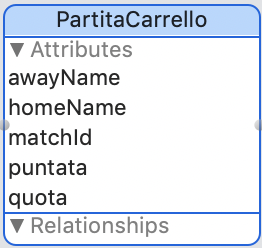
\includegraphics[width=0.2\textwidth]{images/DatiSchedina}
	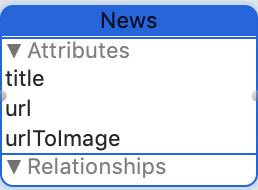
\includegraphics[width=0.2\textwidth]{images/DatiNews}
\end{figure}
In order to purchase the ticket, we used an online database through the Firebase platform. The E / R model used is the follow:
\begin{figure}[H]
	\centering
	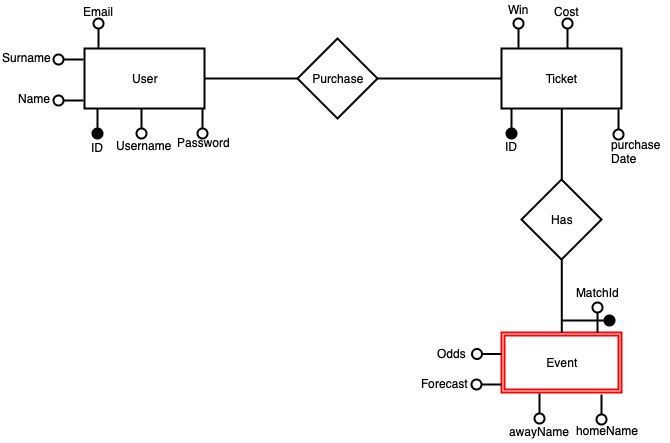
\includegraphics[width=0.7\textwidth]{images/ER.png}
\end{figure}
\newpage
To guarantee privacy, the access to the Database is regulated by the following rules:
\begin{lstlisting}[style=CStyle]
{
	"rules": {
		"Schedina": {
			"$uid": {
				".read": "$uid === auth.uid",
				".write": "$uid === auth.uid"
			}
		}
	}
}
\end{lstlisting}


\section{Client}
For the implementation of the application we have chosen a mobile back-end, that is a client architecture.  This choice was made mainly because the application does not interface with other users and because for various services it uses third-party APIs. Communication with third-party services is based on HTTPS REST requests, in particular through GET requests.\\
The client uses the traditional MVC pattern:
\begin{itemize}
	\item Model: this package contains all the classes representing data to be shown to the single user, taken by the Controller and published by the View.
	\item View: this package contains all the components that display data to the user and interact with him.
	\item Controller: this package contains all the objects in charge to interact between one or more view objects of the application and one or more model objects.
\end{itemize}

\chapter{Use case functional requirements analysis}
This section describes how actors can interact with iSport in order to use all the features implemented in the app. The focus of this part is on the front-end and we show the operations that can be performed by the actors without taking care of the system architecture behind the app.
\begin{figure}[H]
	\centering
	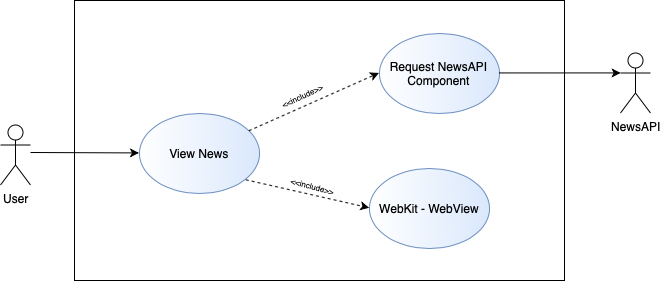
\includegraphics[width=0.7\textwidth]{images/ViewNews}
	\caption{Use case related to visualization and handling news}
\end{figure}
\begin{figure}[H]
	\centering
	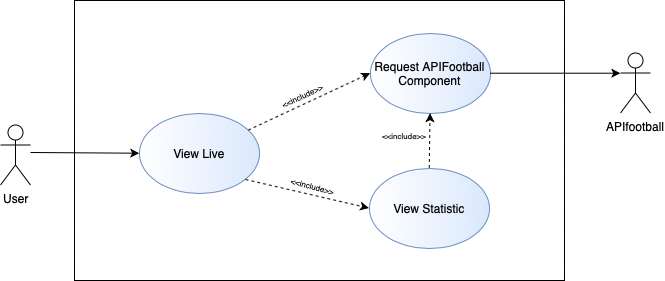
\includegraphics[width=0.7\textwidth]{images/ViewLive}
	\caption{Use case related to visualization and handling results}
\end{figure}
\begin{figure}[H]
	\centering
	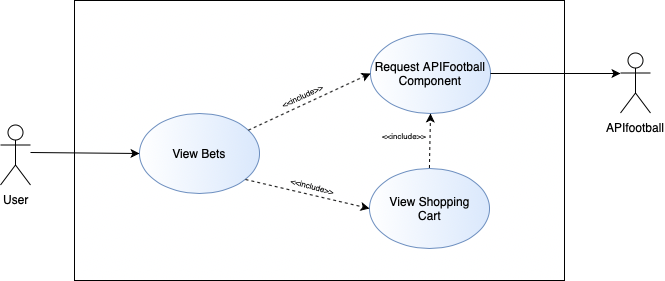
\includegraphics[width=0.7\textwidth]{images/ViewBet}
	\caption{Use case related to visualization and handling odds}
\end{figure}
\begin{figure}[H]
	\centering
	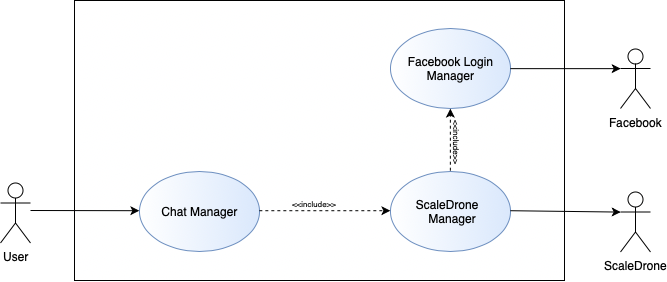
\includegraphics[width=0.7\textwidth]{images/Chat}
	\caption{Use case related to chat service}
\end{figure}
\begin{figure}[H]
	\centering
	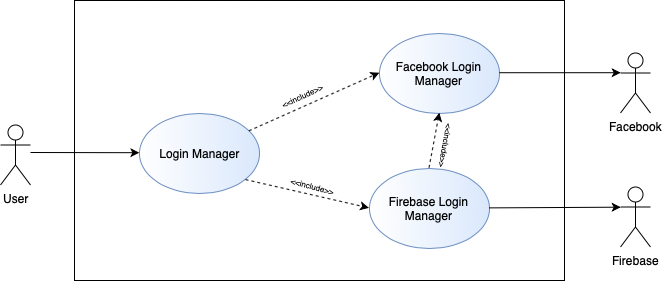
\includegraphics[width=0.7\textwidth]{images/Login}
	\caption{Use case related to log in activity}
\end{figure}
\begin{figure}[H]
	\centering
	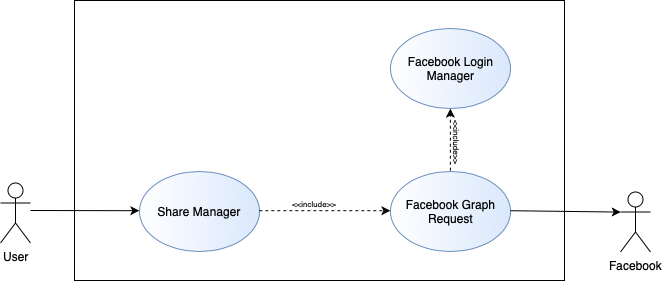
\includegraphics[width=0.7\textwidth]{images/Share}
	\caption{Use case related to news sharing}
\end{figure}
\begin{figure}[H]
	\centering
	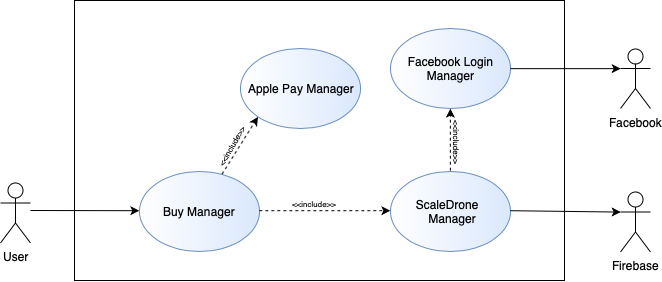
\includegraphics[width=0.7\textwidth]{images/Buy}
	\caption{Use case related to ticket purchase}
\end{figure}
\subsection*{Login}
\begin{tabular}{|c|p{0.8\textwidth}|}
	\hline
	\parbox[c][6ex]{6ex}{\centering \textbf{Name}} & Login\\
	\hline
	\parbox[c][6ex]{6ex}{\centering \textbf{Actor}} & Guest \\
	\hline
	\parbox[c][10ex]{15ex}{\centering \textbf{Entry Condition}} & Guest with login credentials\\
	\hline
	\parbox[c][6ex]{15ex}{\centering \textbf{Goal}} &  14\\
	\hline
	\parbox[c][10ex]{12ex}{\centering \textbf{Event Flow}} & \begin{itemize}
		\item The user opens the application
		\item The user presses ”Login” located in the ”Side Menu”
		\item The user is redirected on Facebook to enter credentials
		\item The app logs in through Facebook
		\item The app login into Firebase using Facebook account
		
	\end{itemize}\\
	\hline
	\parbox[c][7ex]{12ex}{\centering \textbf{Exit condition}} & Actor becomes User \\\hline
	\parbox[c][10ex]{13ex}{\centering \textbf{Exceptions}} & The user is not connected to the network or he hasn’t a Facebook account. \\ \hline	
\end{tabular}
\newpage
\subsection*{Logout}
\begin{tabular}{|c|p{0.8\textwidth}|}
	\hline
	\parbox[c][6ex]{6ex}{\centering \textbf{Name}} & Logout\\
	\hline
	\parbox[c][6ex]{6ex}{\centering \textbf{Actor}} & User \\
	\hline
	\parbox[c][10ex]{15ex}{\centering \textbf{Entry Condition}} & Actor is logged in\\
	\hline
	\parbox[c][6ex]{15ex}{\centering \textbf{Goal}} &  14\\
	\hline
	\parbox[c][10ex]{12ex}{\centering \textbf{Event Flow}} & \begin{itemize}
		\item The user presses ”Logout” located in the ”Side Menu”
		\item The app logout from Facebook
		\item The app logout from Firebase
		
	\end{itemize}\\
	\hline
	\parbox[c][7ex]{12ex}{\centering \textbf{Exit condition}} & Actor is logged out and becomes Guest \\\hline
	\parbox[c][10ex]{13ex}{\centering \textbf{Exceptions}} & The user is not connected to the network. \\ \hline	
\end{tabular}
\newpage
\subsection*{View News}
\begin{tabular}{|c|p{0.8\textwidth}|}
	\hline
	\parbox[c][6ex]{6ex}{\centering \textbf{Name}} & View News\\
	\hline
	\parbox[c][6ex]{6ex}{\centering \textbf{Actor}} & Guest \\
	\hline
	\parbox[c][10ex]{15ex}{\centering \textbf{Entry Condition}} & The user downloaded the mobile app\\
	\hline
	\parbox[c][6ex]{15ex}{\centering \textbf{Goal}} &  1, 2\\
	\hline
	\parbox[c][10ex]{12ex}{\centering \textbf{Event Flow}} & \begin{itemize}
		\item The user opens the app
		\item The user presses on the ”News” tab located to the ”Side Menu”
		\item The app shows a selection of the most important news
		\item The user presses the news to read the whole article
		\item The user presses ”Done” to finish reading
	\end{itemize}\\
	\hline
	\parbox[c][7ex]{12ex}{\centering \textbf{Exit condition}} & The user read the news of interest. \\\hline
	\parbox[c][10ex]{13ex}{\centering \textbf{Exceptions}} &The user is not connected to the network so he cannot send a request to read the article. The news has been released from the origin website, but not from the database. \\ \hline	
\end{tabular}
\newpage
\subsection*{Share News}
\begin{tabular}{|c|p{0.8\textwidth}|}
	\hline
	\parbox[c][6ex]{6ex}{\centering \textbf{Name}} & Share News\\
	\hline
	\parbox[c][6ex]{6ex}{\centering \textbf{Actor}} & User \\
	\hline
	\parbox[c][10ex]{15ex}{\centering \textbf{Entry Condition}} & The user logged in correctly\\
	\hline
	\parbox[c][6ex]{15ex}{\centering \textbf{Goal}} &  11\\
	\hline
	\parbox[c][10ex]{12ex}{\centering \textbf{Event Flow}} & \begin{itemize}
		\item The user opens the app 
		\item The user presses the ”News” tab located in the ”Side Menu”
		\item The app shows a selection of the most important news
		\item The user presses on the ”Share” function 
		\item The user writes the message he wants to attach to the shared post
		\item The user presses ”Publish” 
		
	\end{itemize}\\
	\hline
	\parbox[c][7ex]{12ex}{\centering \textbf{Exit condition}} & The user shares on Facebook the news of interest. \\\hline
	\parbox[c][10ex]{13ex}{\centering \textbf{Exceptions}} & The user is not connected to the network so he cannot send a request to share the article. The news has been released from the origin website, but not from the database or the connection is weak. \\ \hline	
\end{tabular}
\newpage
\subsection*{Save News}
\begin{tabular}{|c|p{0.8\textwidth}|}
	\hline
	\parbox[c][6ex]{6ex}{\centering \textbf{Name}} & Save News\\
	\hline
	\parbox[c][6ex]{6ex}{\centering \textbf{Actor}} & User \\
	\hline
	\parbox[c][10ex]{15ex}{\centering \textbf{Entry Condition}} & The user downloaded the mobile app\\
	\hline
	\parbox[c][6ex]{15ex}{\centering \textbf{Goal}} &  12\\
	\hline
	\parbox[c][10ex]{12ex}{\centering \textbf{Event Flow}} & \begin{itemize}
		\item The user opens the app
		\item The user presses the ”News” tab located in the ”Side Menu”
		\item The app shows a selection of the most important news
		\item The user presses on ”Bookmark” to save the news
		\item The app saves the information in the local database 
		
	\end{itemize}\\
	\hline
	\parbox[c][7ex]{12ex}{\centering \textbf{Exit condition}} & The user saves the news for a following reading. \\\hline
	\parbox[c][10ex]{13ex}{\centering \textbf{Exceptions}} & The user is not connected to the network, so he cannot send a request to save the article. The news has been released from the origin website, but not from the database. \\ \hline	
\end{tabular}
\newpage
\subsection*{See Saved News}
\begin{tabular}{|c|p{0.8\textwidth}|}
	\hline
	\parbox[c][6ex]{6ex}{\centering \textbf{Name}} & See Saved News\\
	\hline
	\parbox[c][6ex]{6ex}{\centering \textbf{Actor}} & User \\
	\hline
	\parbox[c][10ex]{15ex}{\centering \textbf{Entry Condition}} & The user saved the news \\
	\hline
	\parbox[c][6ex]{15ex}{\centering \textbf{Goal}} &  1, 2, 12\\
	\hline
	\parbox[c][10ex]{12ex}{\centering \textbf{Event Flow}} & \begin{itemize}
		\item The user opens the app
		\item The user presses the ”News” tab located in the ”Side Menu”
		\item The user presses on “Bookmark” in the Navigation Bar to see saved news 
		\item The app shows a list of the saved news
	\end{itemize}\\
	\hline
	\parbox[c][7ex]{12ex}{\centering \textbf{Exit condition}} & The user read the news of interest. \\\hline
	\parbox[c][10ex]{13ex}{\centering \textbf{Exceptions}} & The user is not connected to the network so he cannot send a request to read the article. The news has been released from the origin website, but not from the database. \\ \hline	
\end{tabular}
\newpage
\subsection*{See Matches}
\begin{tabular}{|c|p{0.8\textwidth}|}
	\hline
	\parbox[c][6ex]{6ex}{\centering \textbf{Name}} & See Matches\\
	\hline
	\parbox[c][6ex]{6ex}{\centering \textbf{Actor}} & Guest \\
	\hline
	\parbox[c][10ex]{15ex}{\centering \textbf{Entry Condition}} & 
	The user downloaded the app\\
	\hline
	\parbox[c][6ex]{15ex}{\centering \textbf{Goal}} &  3\\
	\hline
	\parbox[c][10ex]{12ex}{\centering \textbf{Event Flow}} & \begin{itemize}
		\item The user opens the app
		\item The user presses the ”Live” tab located in the ”Side Menu”
		\item The app shows a list of matches
		
	\end{itemize}\\
	\hline
	\parbox[c][7ex]{12ex}{\centering \textbf{Exit condition}} & The user saw scores. \\\hline
	\parbox[c][10ex]{13ex}{\centering \textbf{Exceptions}} & The user is not connected to the network, so he cannot send a request to obtain the final scores. \\ \hline	
\end{tabular}



\newpage
\subsection*{View Lineup}
\begin{tabular}{|c|p{0.8\textwidth}|}
	\hline
	\parbox[c][6ex]{6ex}{\centering \textbf{Name}} & View Lineup\\
	\hline
	\parbox[c][6ex]{6ex}{\centering \textbf{Actor}} & Guest \\
	\hline
	\parbox[c][10ex]{15ex}{\centering \textbf{Entry Condition}} & The user downloaded the app\\
	\hline
	\parbox[c][6ex]{15ex}{\centering \textbf{Goal}} &  3, 6\\
	\hline
	\parbox[c][10ex]{12ex}{\centering \textbf{Event Flow}} & \begin{itemize}
		\item The user opens the app
		\item The user presses the ”Live” tab located in the ”Side Menu”
		\item The app shows a list of daily matches 
		\item The user chooses the match to obtain the requested information 
		\item The user presses the button showing the game field 
		
	\end{itemize}\\
	\hline
	\parbox[c][7ex]{12ex}{\centering \textbf{Exit condition}} & The user saw lineups for the requested match  \\\hline
	\parbox[c][10ex]{13ex}{\centering \textbf{Exceptions}} & The user is not connected to the network, so he cannot send a request to obtain results or the connection could be weak.  \\ \hline	
\end{tabular}
\newpage
\subsection*{View Goal Scorer}
\begin{tabular}{|c|p{0.8\textwidth}|}
	\hline
	\parbox[c][6ex]{6ex}{\centering \textbf{Name}} & View Goal Scorer\\
	\hline
	\parbox[c][6ex]{6ex}{\centering \textbf{Actor}} & Guest \\
	\hline
	\parbox[c][10ex]{15ex}{\centering \textbf{Entry Condition}} & The user downloaded the app\\
	\hline
	\parbox[c][6ex]{15ex}{\centering \textbf{Goal}} &  3, 4\\
	\hline
	\parbox[c][10ex]{12ex}{\centering \textbf{Event Flow}} & \begin{itemize}
		\item The user opens the app
		\item The user presses the ”Live” tab located in the ”Side Menu”
		\item The app shows a list of daily matches 
		\item The user chooses the match to obtain the requested information 
		\item The user presses the button showing a ball 
	\end{itemize}\\
	\hline
	\parbox[c][7ex]{12ex}{\centering \textbf{Exit condition}} & The user saw the goal scorers of the requested match.  \\\hline
	\parbox[c][10ex]{13ex}{\centering \textbf{Exceptions}} & The user is not connected to the network, so he cannot send a request to obtain results or the connection could be weak. \\ \hline	
\end{tabular}
\newpage
\subsection*{View Match Statistics}
\begin{tabular}{|c|p{0.8\textwidth}|}
	\hline
	\parbox[c][6ex]{6ex}{\centering \textbf{Name}} & View Match Statistics\\
	\hline
	\parbox[c][6ex]{6ex}{\centering \textbf{Actor}} & Guest \\
	\hline
	\parbox[c][10ex]{15ex}{\centering \textbf{Entry Condition}} & The user downloaded the app\\
	\hline
	\parbox[c][6ex]{15ex}{\centering \textbf{Goal}} &  3, 7\\
	\hline
	\parbox[c][10ex]{12ex}{\centering \textbf{Event Flow}} & \begin{itemize}
		\item The user opens the app
		\item The user presses the ”Live” tab located in the ”Side Menu”
		\item The app shows a list of daily matches 
		\item The user chooses the match to obtain the requested information 
		\item The user presses the button showing a chart
	\end{itemize}\\
	\hline
	\parbox[c][7ex]{12ex}{\centering \textbf{Exit condition}} & The user saw the match statistics. \\\hline
	\parbox[c][10ex]{13ex}{\centering \textbf{Exceptions}} & The user is not connected to the network, so he cannot send a request to obtain results or the connection could be weak. \\ \hline	
\end{tabular}
\newpage
\subsection*{View Match Booking (Cautions)}
\begin{tabular}{|c|p{0.8\textwidth}|}
	\hline
	\parbox[c][6ex]{6ex}{\centering \textbf{Name}} & View Match Booking (Cautions)\\
	\hline
	\parbox[c][6ex]{6ex}{\centering \textbf{Actor}} & Guest \\
	\hline
	\parbox[c][10ex]{15ex}{\centering \textbf{Entry Condition}} & The user downloaded the app\\
	\hline
	\parbox[c][6ex]{15ex}{\centering \textbf{Goal}} &  3, 5\\
	\hline
	\parbox[c][10ex]{12ex}{\centering \textbf{Event Flow}} & \begin{itemize}
		\item The user opens the app
		\item The user presses the ”Live” tab located in the ”Side Menu”
		\item The app shows a list of daily matches 
		\item The user chooses the match to obtain the requested information 
		\item The user presses the button showing a card
	\end{itemize}\\
	\hline
	\parbox[c][7ex]{12ex}{\centering \textbf{Exit condition}} & The user saw booked and expelled players. \\\hline
	\parbox[c][10ex]{13ex}{\centering \textbf{Exceptions}} & The user is not connected to the network, so he cannot send a request to obtain results or the connection could be weak.  \\ \hline	
\end{tabular}
\newpage
\subsection*{View Odds}
\begin{tabular}{|c|p{0.8\textwidth}|}
	\hline
	\parbox[c][6ex]{6ex}{\centering \textbf{Name}} & View Odds\\
	\hline
	\parbox[c][6ex]{6ex}{\centering \textbf{Actor}} & Guest \\
	\hline
	\parbox[c][10ex]{15ex}{\centering \textbf{Entry Condition}} & The user downloaded the app\\
	\hline
	\parbox[c][6ex]{15ex}{\centering \textbf{Goal}} &  8\\
	\hline
	\parbox[c][10ex]{12ex}{\centering \textbf{Event Flow}} & \begin{itemize}
		\item The user opens the app
		\item The user presses the “Bet” tab located in the ”Side Menu”
		\item The app shows a list of principle odds of the daily matches 
		
	\end{itemize}\\
	\hline
	\parbox[c][7ex]{12ex}{\centering \textbf{Exit condition}} & The user saw the odds of the daily matches. \\\hline
	\parbox[c][10ex]{13ex}{\centering \textbf{Exceptions}} & The user is not connected to the network, so he cannot send a request to obtain results or the connection could be weak.  \\ \hline	
\end{tabular}
\newpage
\subsection*{View Ticket}
\begin{tabular}{|c|p{0.8\textwidth}|}
	\hline
	\parbox[c][6ex]{6ex}{\centering \textbf{Name}} & View Ticket\\
	\hline
	\parbox[c][6ex]{6ex}{\centering \textbf{Actor}} & Guest \\
	\hline
	\parbox[c][10ex]{15ex}{\centering \textbf{Entry Condition}} & The user downloaded the app\\
	\hline
	\parbox[c][6ex]{15ex}{\centering \textbf{Goal}} &  9\\
	\hline
	\parbox[c][10ex]{12ex}{\centering \textbf{Event Flow}} & \begin{itemize}
		\item The user opens the app
		\item The user presses the “Bet” tab located in the ”Side Menu”
		\item The user presses the button showing a cart 
	\end{itemize}\\
	\hline
	\parbox[c][7ex]{12ex}{\centering \textbf{Exit condition}} & The user sees the ticket.\\\hline
	\parbox[c][10ex]{13ex}{\centering \textbf{Exceptions}} & The user is not connected to the network, so he cannot send a request to obtain results or the connection could be weak. \\ \hline	
\end{tabular}
\newpage
\subsection*{Add Match To The Ticket }
\begin{tabular}{|c|p{0.8\textwidth}|}
	\hline
	\parbox[c][6ex]{6ex}{\centering \textbf{Name}} & Add Match To The Ticket\\
	\hline
	\parbox[c][6ex]{6ex}{\centering \textbf{Actor}} & Guest \\
	\hline
	\parbox[c][10ex]{15ex}{\centering \textbf{Entry Condition}} & The user downloaded the app \\
	\hline
	\parbox[c][6ex]{15ex}{\centering \textbf{Goal}} &  9\\
	\hline
	\parbox[c][10ex]{12ex}{\centering \textbf{Event Flow}} & \begin{itemize}
		\item The user opens the app
		\item The user presses the “Bet” tab located in the ”Side Menu”
		\item The app shows a list of principle odds of the daily matches 
		\item The user presses on the odd and add the forecast to the ticket
		
	\end{itemize}\\
	\hline
	\parbox[c][7ex]{12ex}{\centering \textbf{Exit condition}} & The user added a forecast to the ticket.\\\hline
	\parbox[c][10ex]{13ex}{\centering \textbf{Exceptions}} & The user is not connected to the network, so he cannot send a request to obtain results or the connection could be weak. \\ \hline	
\end{tabular}
\newpage
\subsection*{Delete a Match}
\begin{tabular}{|c|p{0.8\textwidth}|}
	\hline
	\parbox[c][6ex]{6ex}{\centering \textbf{Name}} & Delete a Match\\
	\hline
	\parbox[c][6ex]{6ex}{\centering \textbf{Actor}} & Guest \\
	\hline
	\parbox[c][10ex]{15ex}{\centering \textbf{Entry Condition}} & The user downloaded the app\\
	\hline
	\parbox[c][6ex]{15ex}{\centering \textbf{Goal}} &  9\\
	\hline
	\parbox[c][10ex]{12ex}{\centering \textbf{Event Flow}} & \begin{itemize}
		\item The user opens the app
		\item The user presses the “Bet” tab located in the ”Side Menu”
		\item The user presses the button showing a cart
		\item The user swipes to the left to delete the match 
	\end{itemize}\\
	\hline
	\parbox[c][7ex]{12ex}{\centering \textbf{Exit condition}} & The user deleted a forecast from the ticket \\\hline
	\parbox[c][10ex]{13ex}{\centering \textbf{Exceptions}} & None\\ \hline	
\end{tabular}
\newpage
\subsection*{Calculate The Potential Winning}
\begin{tabular}{|c|p{0.8\textwidth}|}
	\hline
	\parbox[c][6ex]{6ex}{\centering \textbf{Name}} & Calculate The Potential Winning\\
	\hline
	\parbox[c][6ex]{6ex}{\centering \textbf{Actor}} & Guest \\
	\hline
	\parbox[c][10ex]{15ex}{\centering \textbf{Entry Condition}} & The user downloaded the app\\
	\hline
	\parbox[c][6ex]{15ex}{\centering \textbf{Goal}} &  10\\
	\hline
	\parbox[c][10ex]{12ex}{\centering \textbf{Event Flow}} & \begin{itemize}
		\item The user opens the app
		\item The user presses the “Bet” tab located in the ”Side Menu”
		\item The user presses the button showing a cart
		\item The user selects the amount of money he wants to bet 
		\item The user presses on “Done”
		
	\end{itemize}\\
	\hline
	\parbox[c][7ex]{12ex}{\centering \textbf{Exit condition}} & The user sees the potential winning \\\hline
	\parbox[c][10ex]{13ex}{\centering \textbf{Exceptions}} & None \\ \hline	
\end{tabular}
\newpage
\subsection*{Purchase ticket}
\begin{tabular}{|c|p{0.8\textwidth}|}
	\hline
	\parbox[c][6ex]{6ex}{\centering \textbf{Name}} & Purchase ticket\\
	\hline
	\parbox[c][6ex]{6ex}{\centering \textbf{Actor}} & User \\
	\hline
	\parbox[c][10ex]{15ex}{\centering \textbf{Entry Condition}} & The user logged in correctly \\
	\hline
	\parbox[c][6ex]{15ex}{\centering \textbf{Goal}} &  9, 10\\
	\hline
	\parbox[c][10ex]{12ex}{\centering \textbf{Event Flow}} & \begin{itemize}
		\item The user opens the app
		\item The user presses the “Bet” tab located in the ”Side Menu”
		\item The user presses the button showing a cart
		\item The user selects the amount of money he wants to bet 
		\item The user presses on ”Buy”
		
	\end{itemize}\\
	\hline
	\parbox[c][7ex]{12ex}{\centering \textbf{Exit condition}} & The user completes the purchase.\\\hline
	\parbox[c][10ex]{13ex}{\centering \textbf{Exceptions}} & Absent connection to the network, the user cannot complete the purchase. The user didn’t log correctly or he didn’t add matches to the ticket.  \\ \hline	
\end{tabular}
\newpage
\subsection*{View Purchased Tickets}
\begin{tabular}{|c|p{0.8\textwidth}|}
	\hline
	\parbox[c][6ex]{6ex}{\centering \textbf{Name}} & View Purchased Tickets\\
	\hline
	\parbox[c][6ex]{6ex}{\centering \textbf{Actor}} & User \\
	\hline
	\parbox[c][10ex]{15ex}{\centering \textbf{Entry Condition}} & The user logged in correctly\\
	\hline
	\parbox[c][6ex]{15ex}{\centering \textbf{Goal}} &  9, 10\\
	\hline
	\parbox[c][10ex]{12ex}{\centering \textbf{Event Flow}} & \begin{itemize}
		\item The user opens the app
		\item The user presses the “Bet” tab located in the ”Side Menu”
		\item The user presses on “chronology” in the NavBar
		\item The app downloads the information about all purchased tickets 
		\item The user presses on the corresponding cell of the ticket he wants to see 
		\item The app loads the ticket and the user sees all the details 
	\end{itemize}\\
	\hline
	\parbox[c][7ex]{12ex}{\centering \textbf{Exit condition}} & The user sees a purchased ticket previously.\\\hline
	\parbox[c][10ex]{13ex}{\centering \textbf{Exceptions}} & The user is not connected to the network, so he cannot send a request to obtain results or the connection could be weak. The user didn’t log correctly or he didn’t buy a ticket. \\ \hline	
\end{tabular}
\newpage
\subsection*{Chat}
\begin{tabular}{|c|p{0.8\textwidth}|}
	\hline
	\parbox[c][6ex]{6ex}{\centering \textbf{Name}} & Chat\\
	\hline
	\parbox[c][6ex]{6ex}{\centering \textbf{Actor}} & User \\
	\hline
	\parbox[c][10ex]{15ex}{\centering \textbf{Entry Condition}} & The user logged in correctly \\
	\hline
	\parbox[c][6ex]{15ex}{\centering \textbf{Goal}} &  13\\
	\hline
	\parbox[c][10ex]{12ex}{\centering \textbf{Event Flow}} & \begin{itemize}
		\item The user opens the app
		\item The user presses the “Chat” tab located in the ”Side Menu”
		\item The app logs into Scaledrone’s room using Facebook credentials  
		\item The user writes messages in the text field 
		\item The user presses send 
		\item The app loads all the messages of the room 
		
	\end{itemize}\\
	\hline
	\parbox[c][7ex]{12ex}{\centering \textbf{Exit condition}} & The user interacts with other people. \\\hline
	\parbox[c][10ex]{13ex}{\centering \textbf{Exceptions}} & The user is not connected or he has not a Facebook account.\\ \hline	
\end{tabular}
\newpage


\chapter{Sequence Diagram}
In order to explain our work and facilitate further implementations we have decided to show the logical flows aimed to create some features. The sequence diagrams will describe the interactions between the different parts of the system and the user.

\subsection*{Login}
The ”Login” procedure starts when the user presses the button on the Side Menu.  Once pressed, the user is redirected to the Facebook site to complete the registration. Immediately after logging on Facebook the application will log into the Firebase Database.

Once this procedure is completed, the system will update the GUI by enabling the sections available only to subscribers.

In the event of an error, the system will show an error message.

\begin{figure}[H]
	\centering
	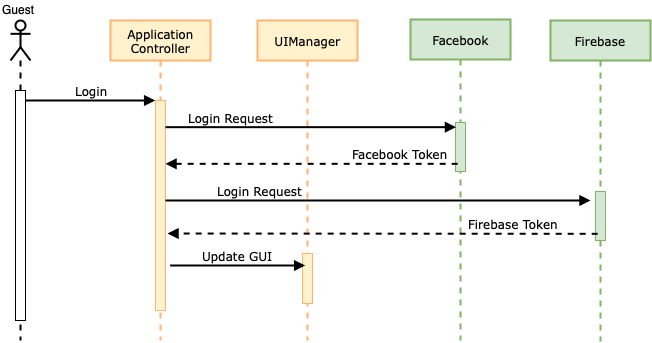
\includegraphics[width=1\textwidth]{images/Sequence/Login}
\end{figure}
\newpage

\subsection*{Logout}
The ”Logout” procedure starts when the user presses the button on the Side Menu. Once pressed, a confirmation message will be displayed. In case of approval, the logout from Facebook and Firebase will be effective.

Now that this procedure is completed, the system will update the GUI by enabling sections not available for guests.


\begin{figure}[H]
	\centering
	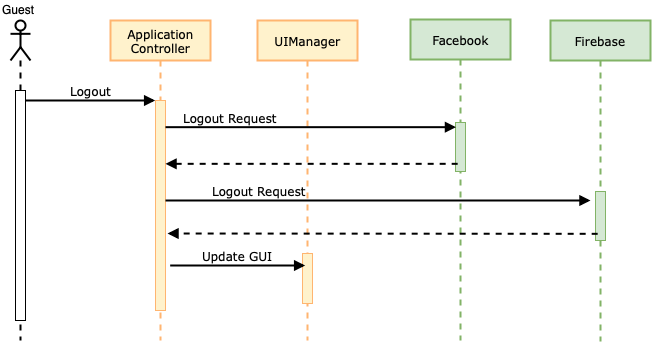
\includegraphics[width=1\textwidth]{images/Sequence/Logout}
\end{figure}
\newpage


\subsection*{View News}
The ”View News” procedure starts when the user opens the application or presses the ”News” section in the Tab Navigator. The sequence diagram shows the normal procedure.

After the user activates the News section, the application will send a request to the ”NewsAPI” service in order to obtain all the information related to the most important daily news.

Once this information is obtained, the Controller will create a UITableViewCell for each news and insert them into the TableView.

Furthermore and asynchronously, the application will download the preview images to allow the user to read the news headlines. When a cell is pressed the Controller will open a WebView addressed to the URL of the news in order to allow the user to read  the complete article.

\begin{figure}[H]
	\centering
	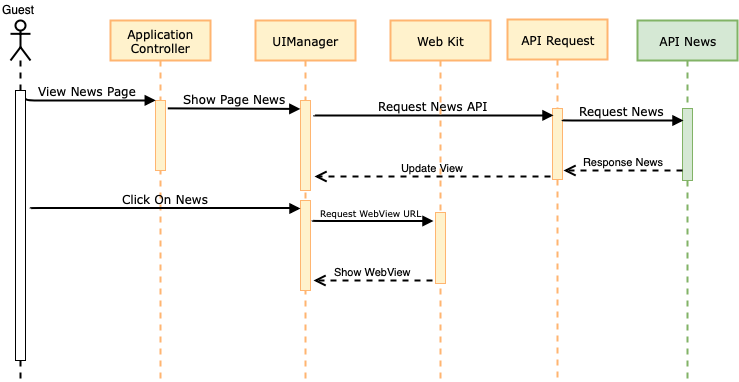
\includegraphics[width=1\textwidth]{images/Sequence/SequenceNews}
\end{figure}


\newpage

\subsection*{Share News}
The ”Share News” procedure starts when the user opens the application or presses ”News” on the Side Menu. The sequence diagram shows the normal procedure.

After the normal ”View News” procedure the user should press the share button. At that point the application will make a request to the ”Graph” API of Facebook to create the post with the message entered by the user.

To make this operation possible is necessary that the user is already authenticated otherwise the system will show an error notice.


\begin{figure}[H]
	\centering
	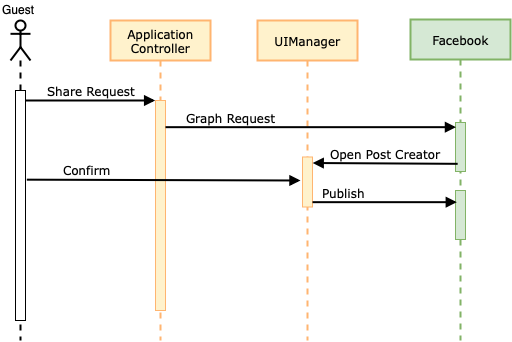
\includegraphics[width=1\textwidth]{images/Sequence/SharePost}
\end{figure}


\newpage



\subsection*{View Match}
The ”View Match” procedure starts when the user presses the “Live” section of the Tab Bar Navigator.

After activating the ”Live” section, the application will send a request to the ”API- Football” service to obtain information about the daily matches and their forecasts.

When this information has been reached, the Controller will create a UITableViewCell for all the matches and insert them into the TableView.

At regular intervals the Controller will repeat these requests to keep the matches updated.

\begin{figure}[H]
	\centering
	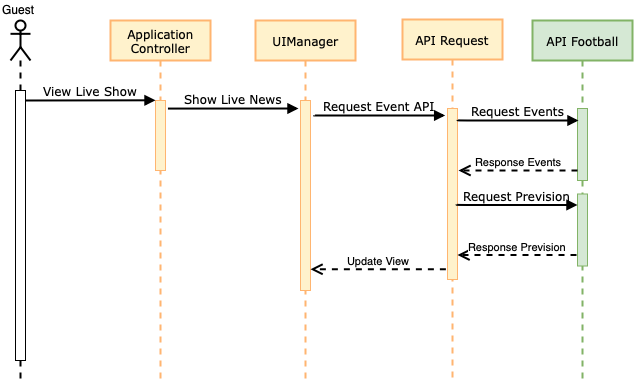
\includegraphics[width=1\textwidth]{images/Sequence/SequenceLive}
\end{figure}


\newpage
\subsection*{View Match Details}
The ”View Match” procedure starts when the user is in the ”Live” section and presses on a single match to know the details.

Now the Controller has access to the data for the specific match, previously downloaded from the “APIFootball” service and creates Views for every information. 

After opening the detail page, the user can change the desired information through the relative buttons.

\begin{figure}[H]
	\centering
	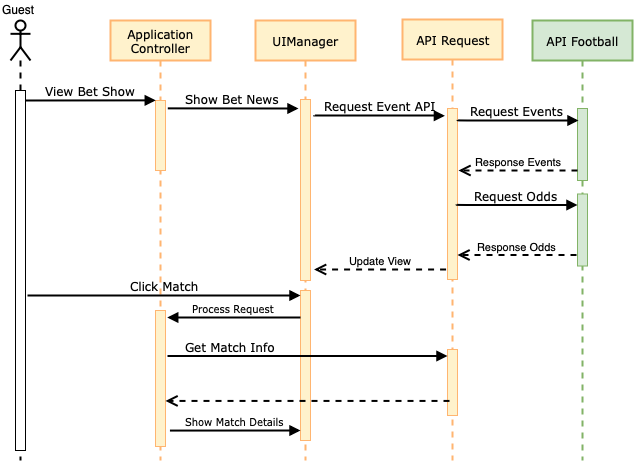
\includegraphics[width=1\textwidth]{images/Sequence/SequenceMatchDetails}
\end{figure}

\newpage

\subsection*{Chat}
The ”Chat” procedure starts when the user presses the button on the Side Menu. Once the screen is loaded, the application will show all messages sent by other users in real time. The user can then write and send his message.

The application will also show Facebook profile images of other users next to the message sent.

To make this operation possible is necessary that the user is already authenticated otherwise the system will show an error notice.


\begin{figure}[H]
	\centering
	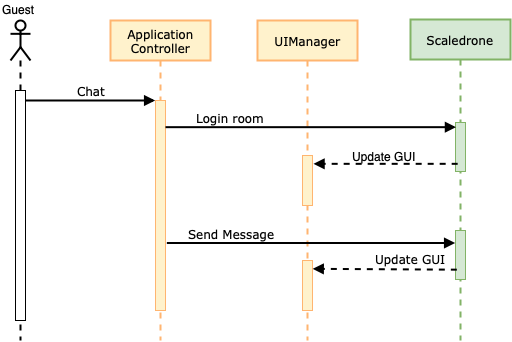
\includegraphics[width=1\textwidth]{images/Sequence/Chat}
\end{figure}
\newpage

\subsection*{View Odds}
The ”View Odds” procedure starts when the user presses the “Bet” section on the Tab Bar Navigator.

Activated the ”Bet” section, the application will send a request to the ”APIFootball” service to obtain information about the daily matches and the relative odds.

At this point, the Controller will create a UITableViewCell for each news and insert them into the TableView. In particular, we inserted three buttons (one for each prediction) with the relative odd indicated.

At regular intervals the Controller will repeat these requests to keep the matches updated.
\begin{figure}[H]
	\centering
	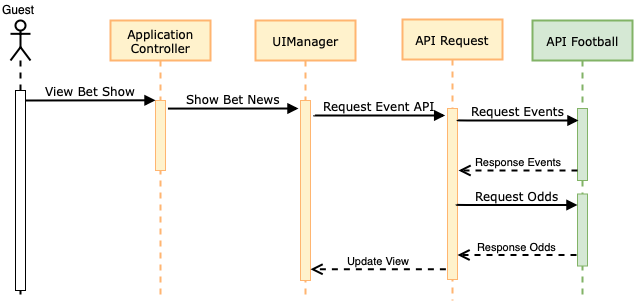
\includegraphics[width=1\textwidth]{images/Sequence/SequenceOdds}
\end{figure}

\newpage
\subsection*{Add Odd}
The ”Add Odd” procedure starts when the user is in the ”Bet” section and presses on  the prediction of the match he wants to bet on.

At that point the Controller has access to the data for the specific match, previously downloaded from the ”APIFootball” service and create the data structure that will be saved in the Database.

Once the data structure is created, the Controller will check if the match is already present in the database; If so, it will update the element with the new forecast, otherwise it will create a new record.

After updating the DB the Controller will update the current View to show the change in a visual feedback.

\begin{figure}[H]
	\centering
	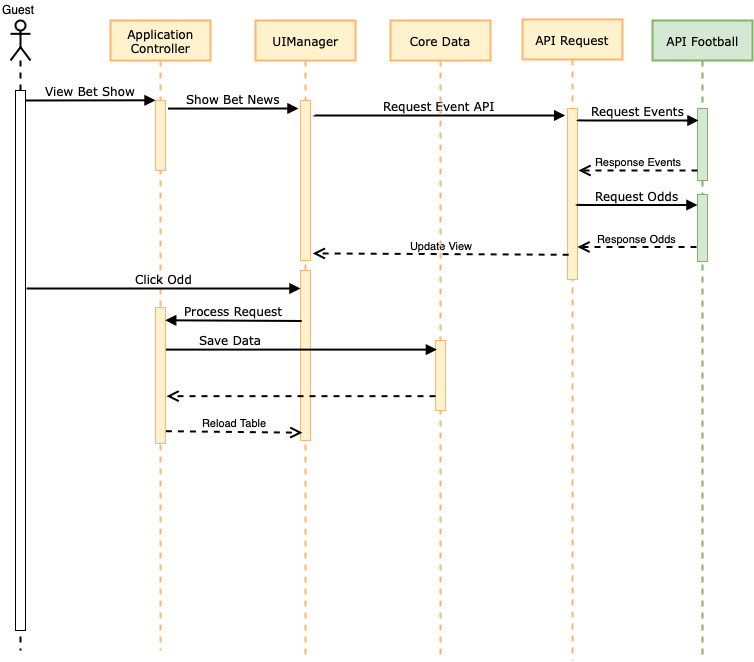
\includegraphics[width=1\textwidth]{images/Sequence/SequenceAddOdd}
\end{figure}
\newpage
\subsection*{View Cart}
The ”View Cart” procedure starts when the user is in the ”Bet” section and presses the button showing a cart in the Navigation bar.

At  that point, the Controller has access to the data in the Database and for each of them  it will create a UITableViewCell to be inserted in the TableView.

The user can change the amount of money gambled  by using the corresponding  input.  Once the amount has been updated, the Controller will calculate the potential winnings by multiplying all the odds with the amount played.

\begin{figure}[H]
	\centering
	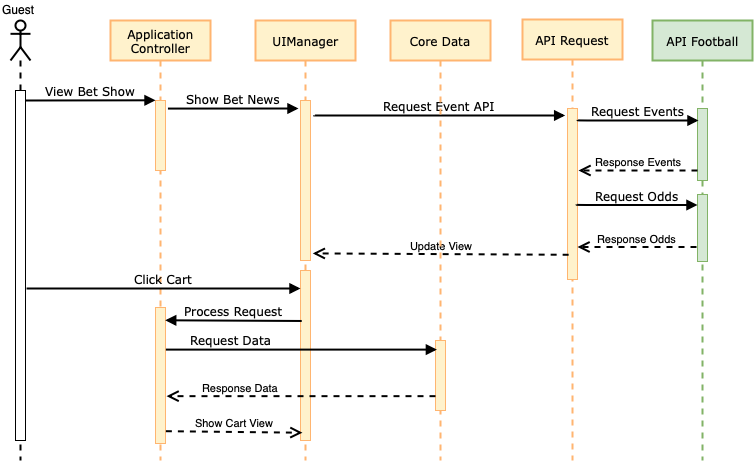
\includegraphics[width=1\textwidth]{images/Sequence/SequenceViewCart}
\end{figure}
\newpage
\subsection*{Remove Odd}
The procedure of  ”Remove Odd” begins when the user is in the ”Bet” section and he is checking the cart.

In this section the user can delete each bet by swiping to the left with his finger.

At that point the Controller will delete the corresponding record from the Database and update the contents of the shopping cart also recalculating the new potential winnings.
\begin{figure}[H]
	\centering
	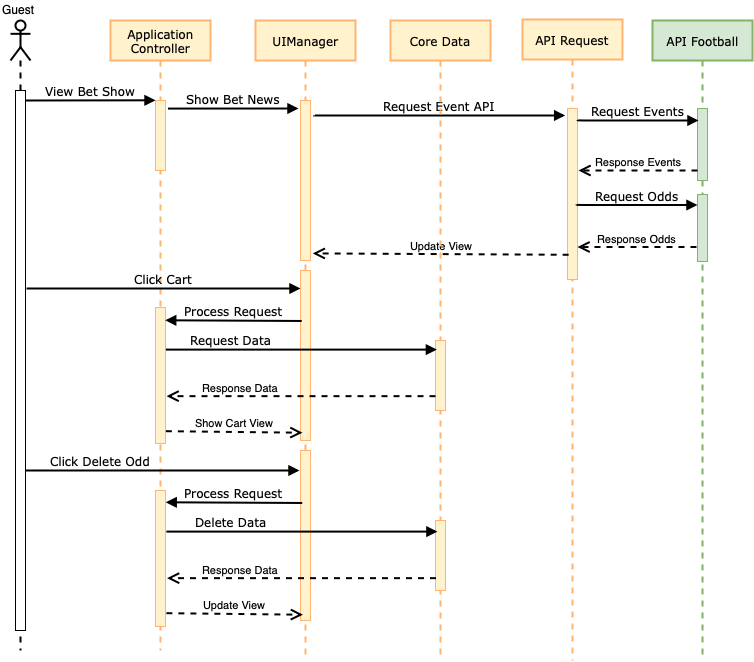
\includegraphics[width=1\textwidth]{images/Sequence/SequenceRemoveOdd}
\end{figure}

\newpage

\subsection*{Buy Ticket}
When the user completes the composition of his ticket, the ”Buy Ticket” procedure may begin.

By pressing the buy button, the application will check the correctness of the ticket and proceed with the purchase.

To make this operation possible is necessary that the user is already authenticated otherwise the system will show an error notice.


\begin{figure}[H]
	\centering
	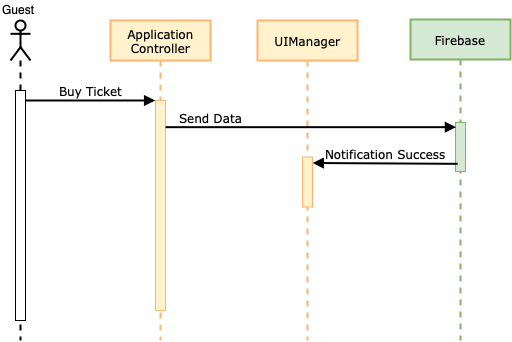
\includegraphics[width=1\textwidth]{images/Sequence/BuyTicket}
\end{figure}

\newpage

\subsection*{Ticket Chronology}
The ”Ticket Chronology” procedure starts when the user is in the ”Bet” section by pressing the button in the Side Menu.

Moreover, by pressing ”History” on the NavBar the application access Firebase database showing all the tickets purchased previously by the user.

To make this procedure possible is necessary that the user is already authenticated otherwise the system will show an error notice.

\begin{figure}[H]
	\centering
	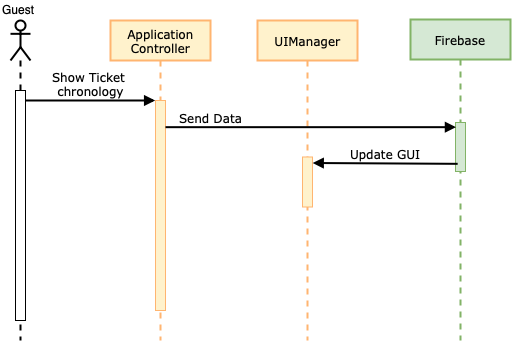
\includegraphics[width=1\textwidth]{images/Sequence/TicketChronology}
\end{figure}


\chapter{User Interfaces}
In this chapter will be discussed and displayed the user interface of each page highlighting the functionalities of the iSport application.
\subsection*{Side Menu}
\begin{figure}[H]
	\begin{subfigure}{.5\textwidth}
		\centering
		\includegraphics[width=.8\linewidth]{images/Screen/SideMenu}
		\caption{This screen shows the Side Menu of an authenticated user}
	\end{subfigure}
	\begin{subfigure}{.5\textwidth}
		\centering
		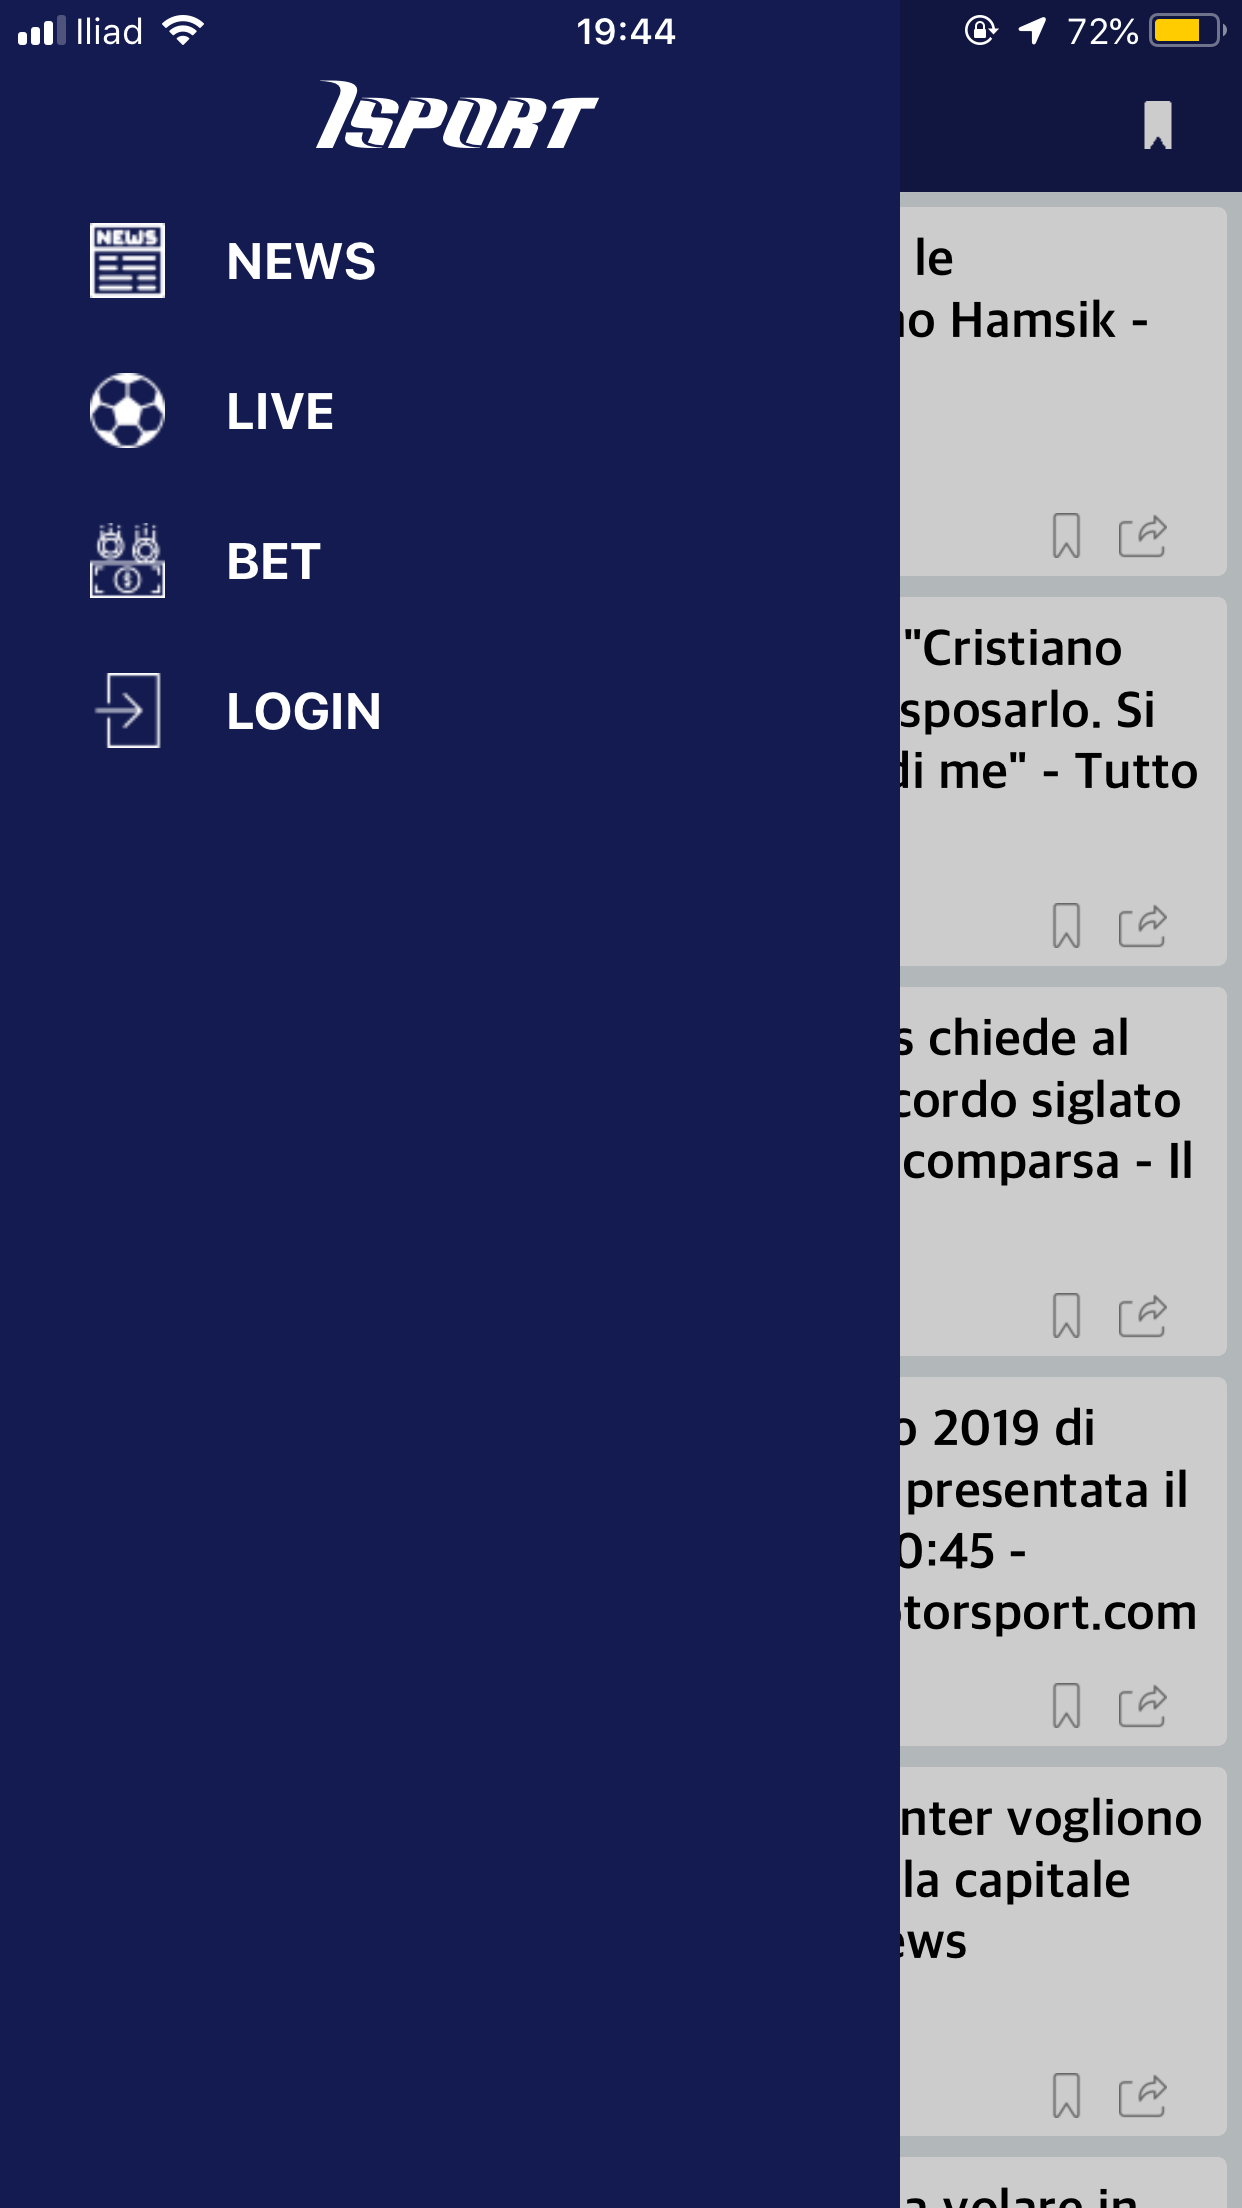
\includegraphics[width=.8\linewidth]{images/Screen/SideLogout}
		\caption{This screen shows the Side Menu of an unauthenticated user}
	\end{subfigure}
\end{figure}



\subsection*{News}

\begin{figure}[H]
	\begin{subfigure}{.5\textwidth}
		\centering
		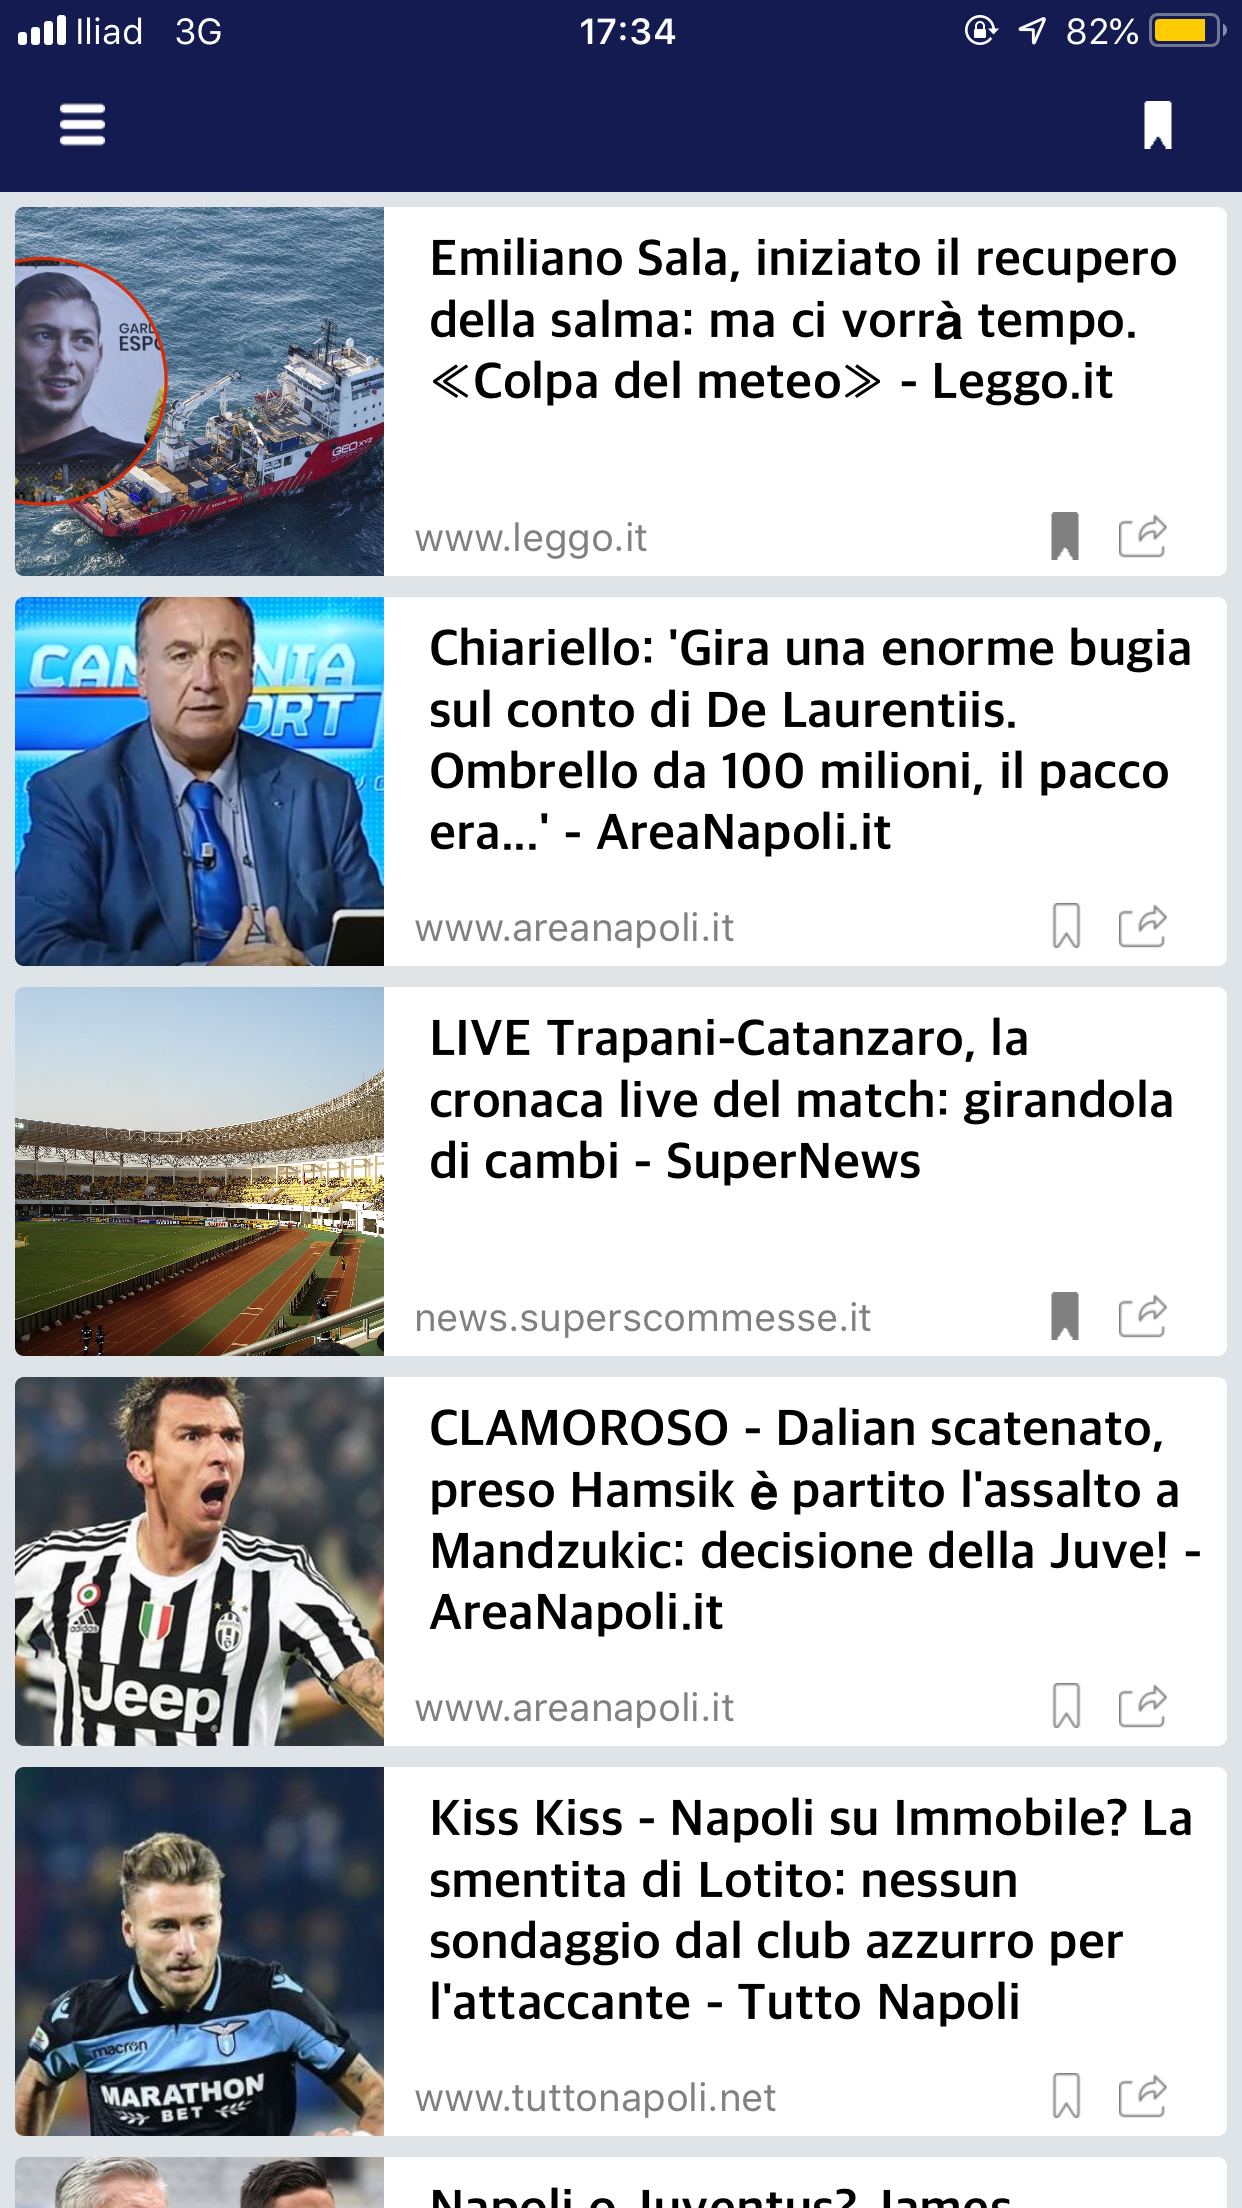
\includegraphics[width=.8\linewidth]{images/Screen/News}
		\caption{This screen shows all the news along with the possibility to save or publish them}
	\end{subfigure}
	\begin{subfigure}{.5\textwidth}
		\centering
		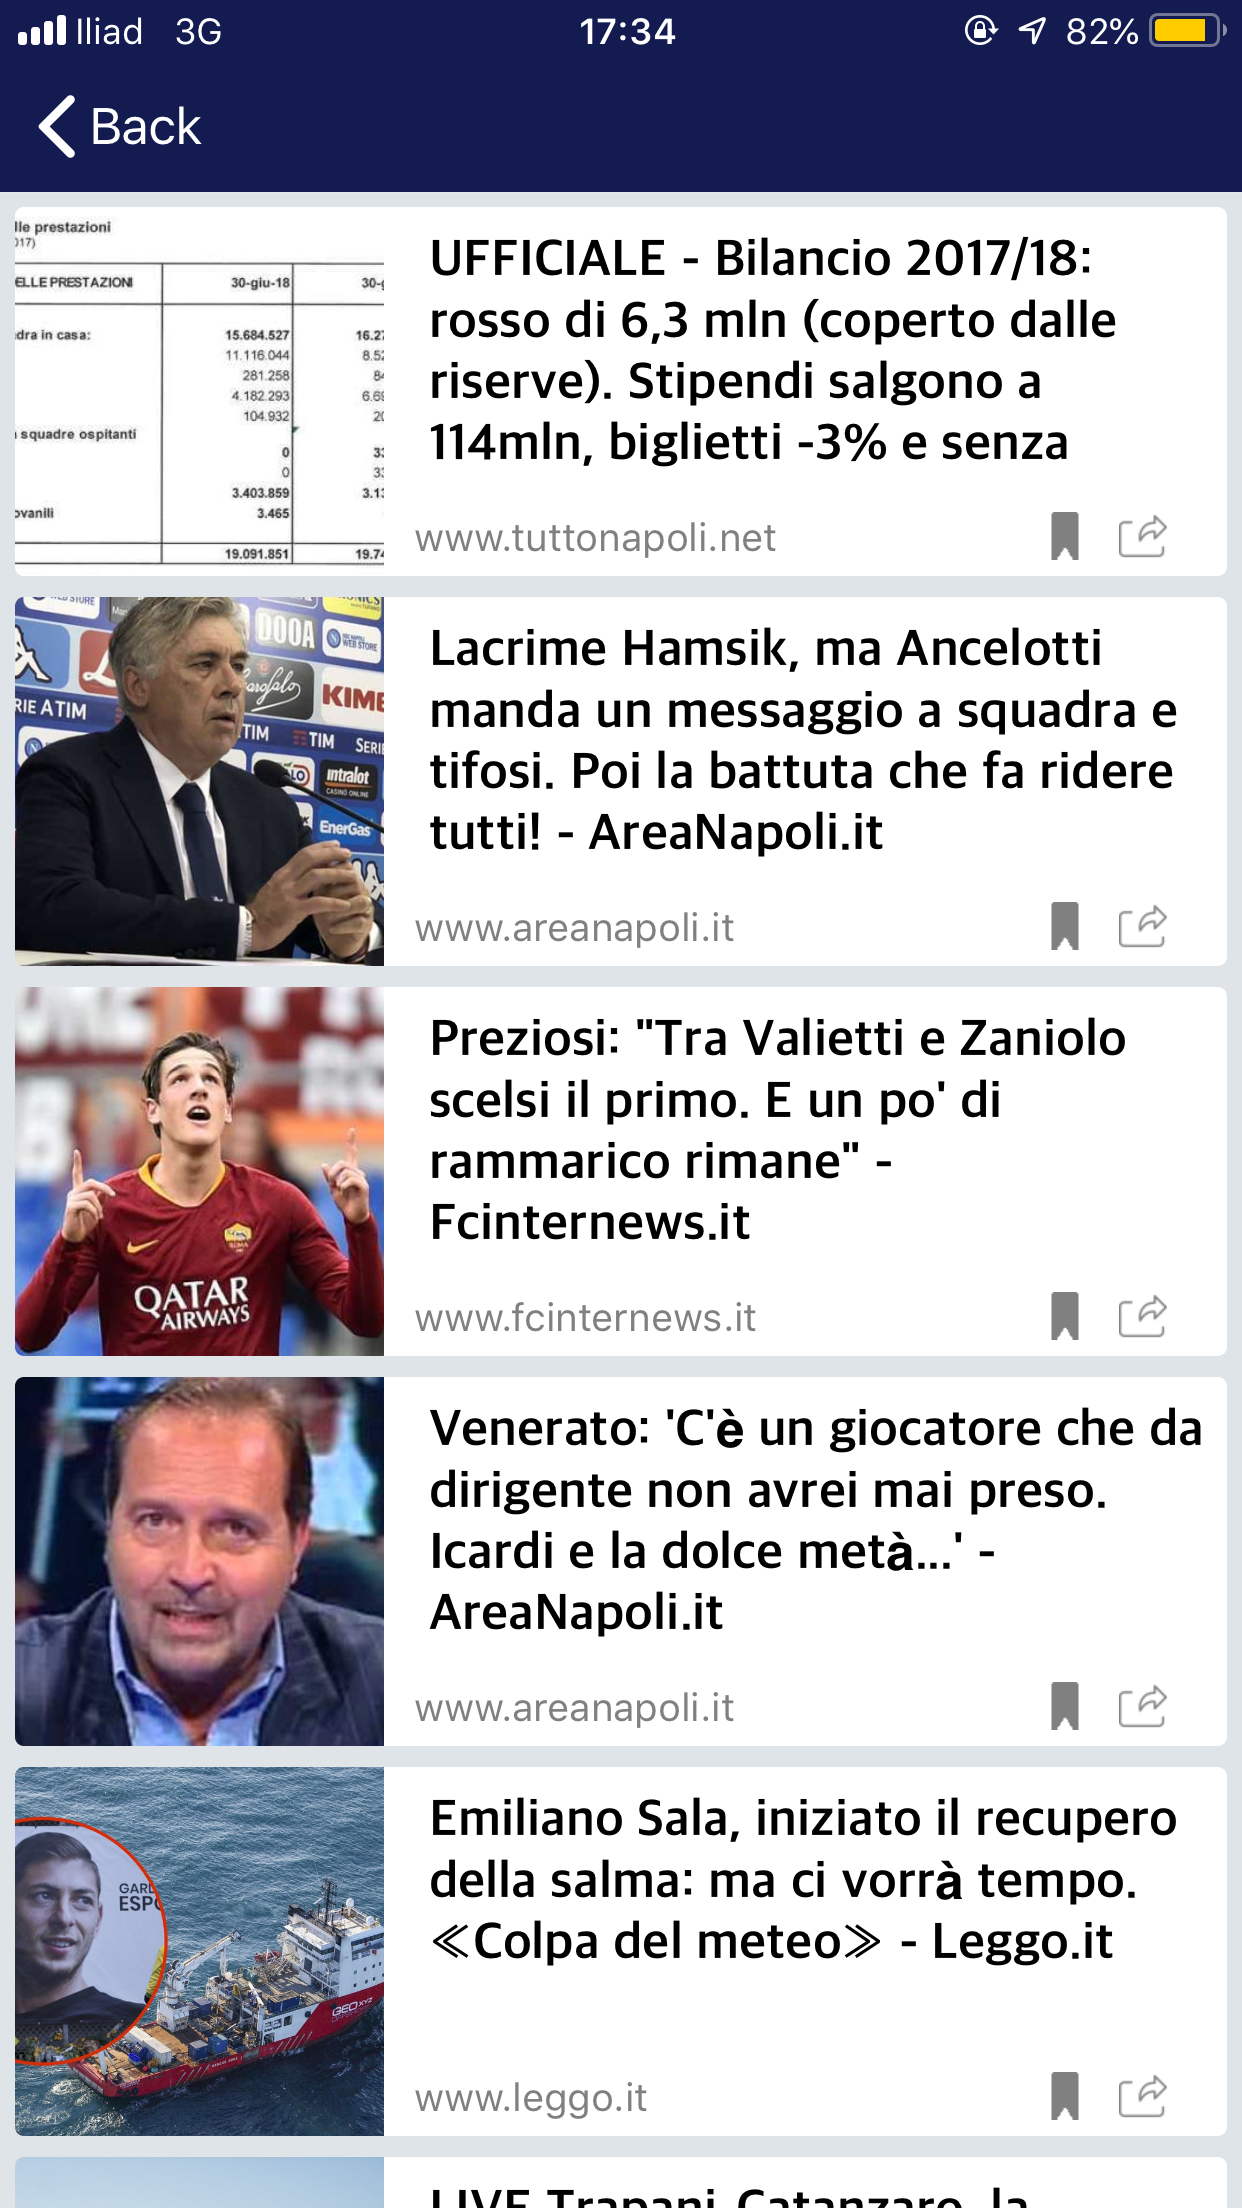
\includegraphics[width=.8\linewidth]{images/Screen/NewsFavorite}
		\caption{This screen shows all the saved news}
	\end{subfigure}
\end{figure}

\begin{figure}[H]
		\begin{subfigure}{.5\textwidth}
		\centering
		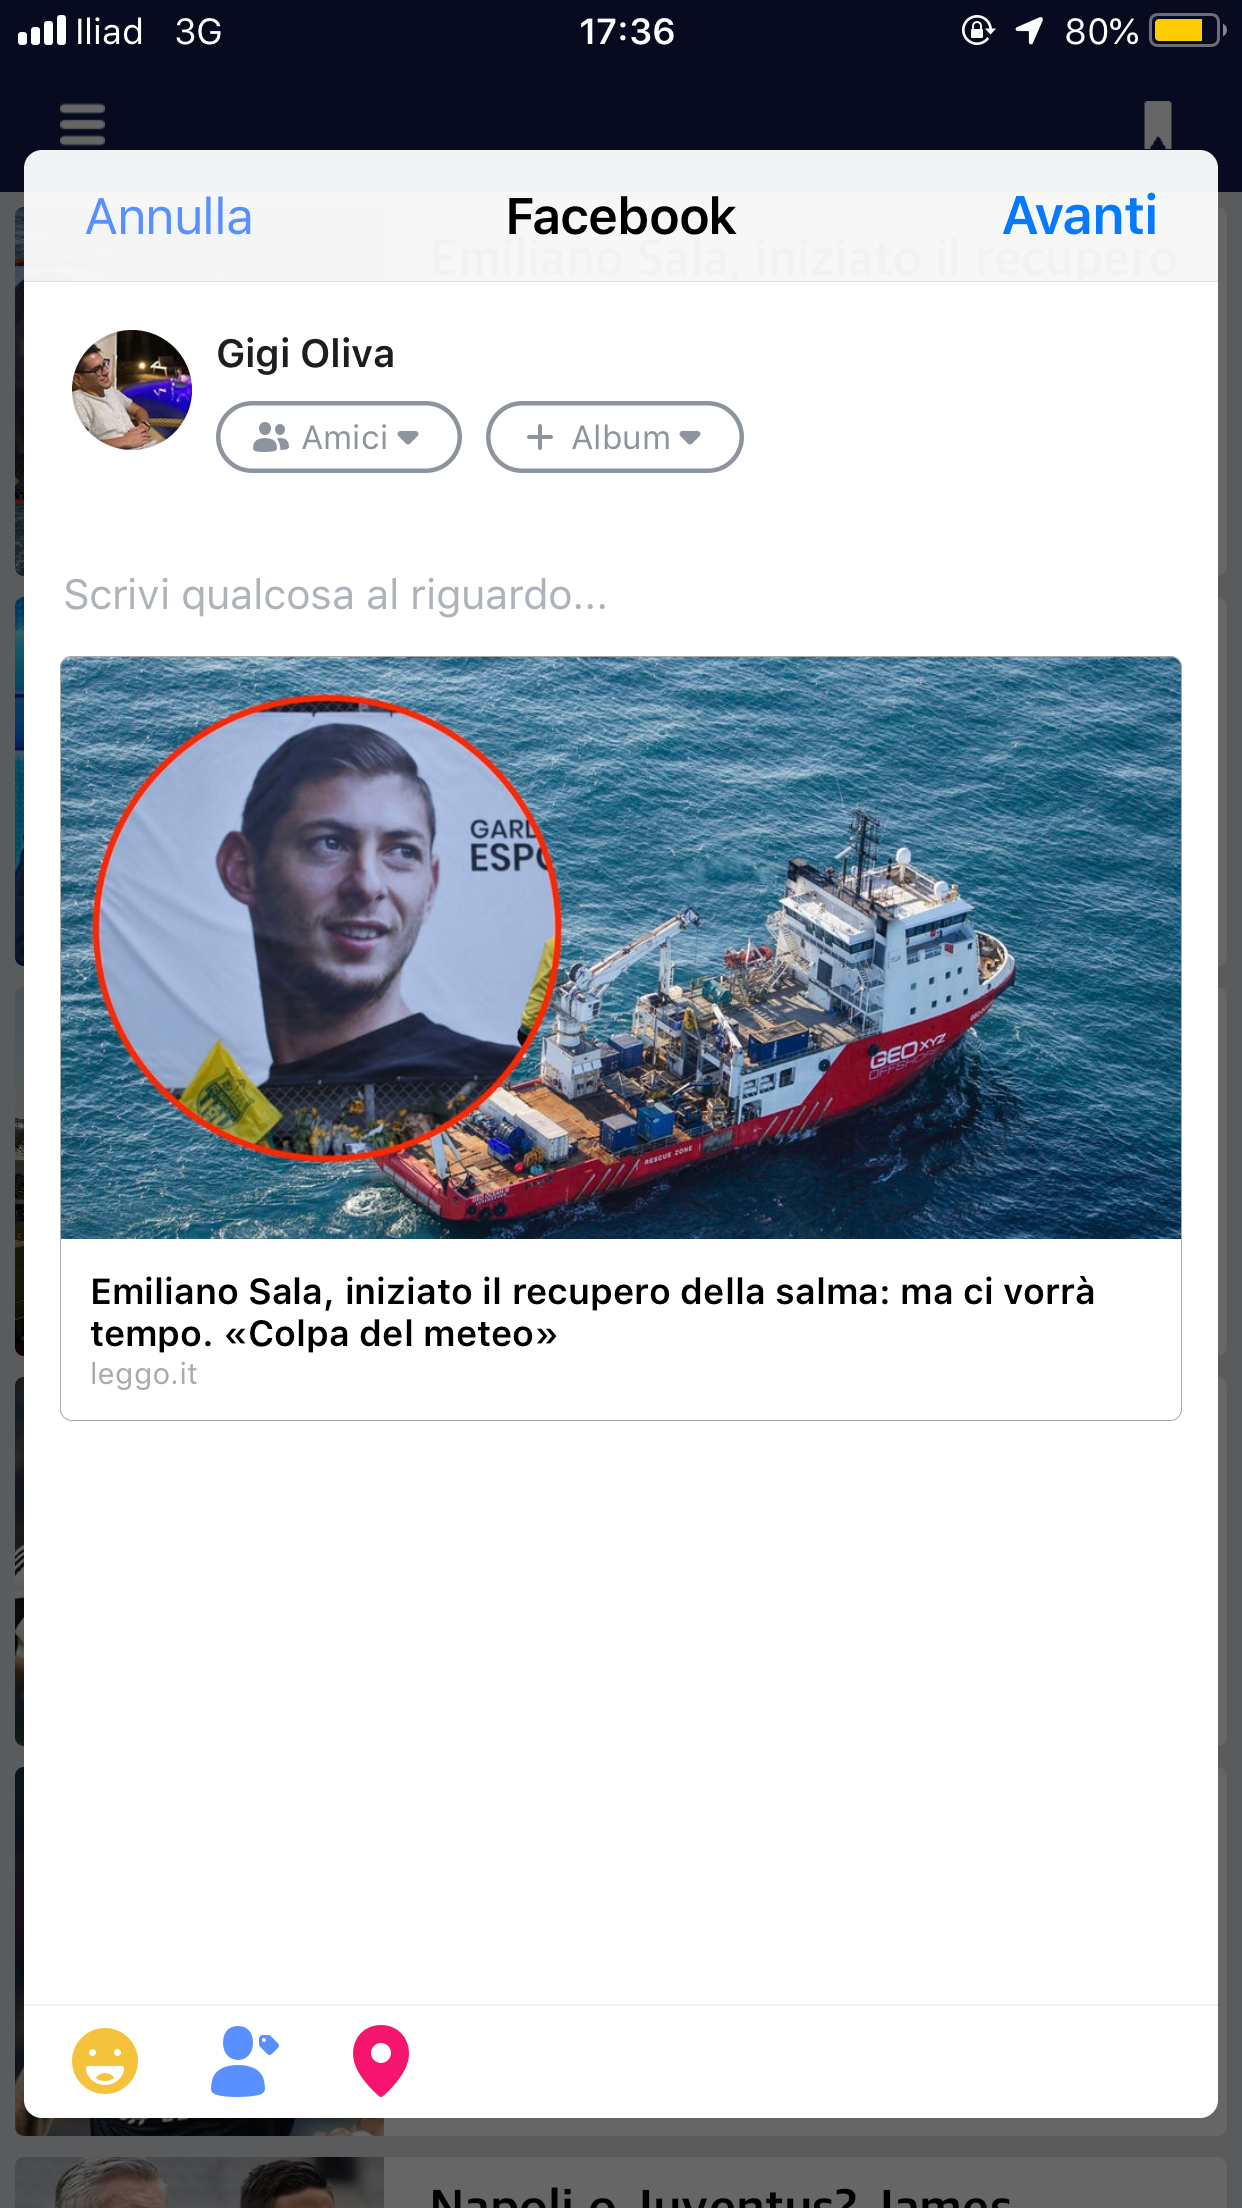
\includegraphics[width=.8\linewidth]{images/Screen/Share}
		\caption{This screen shows the News sharing}
	\end{subfigure}
	\begin{subfigure}{.5\textwidth}
		\centering
		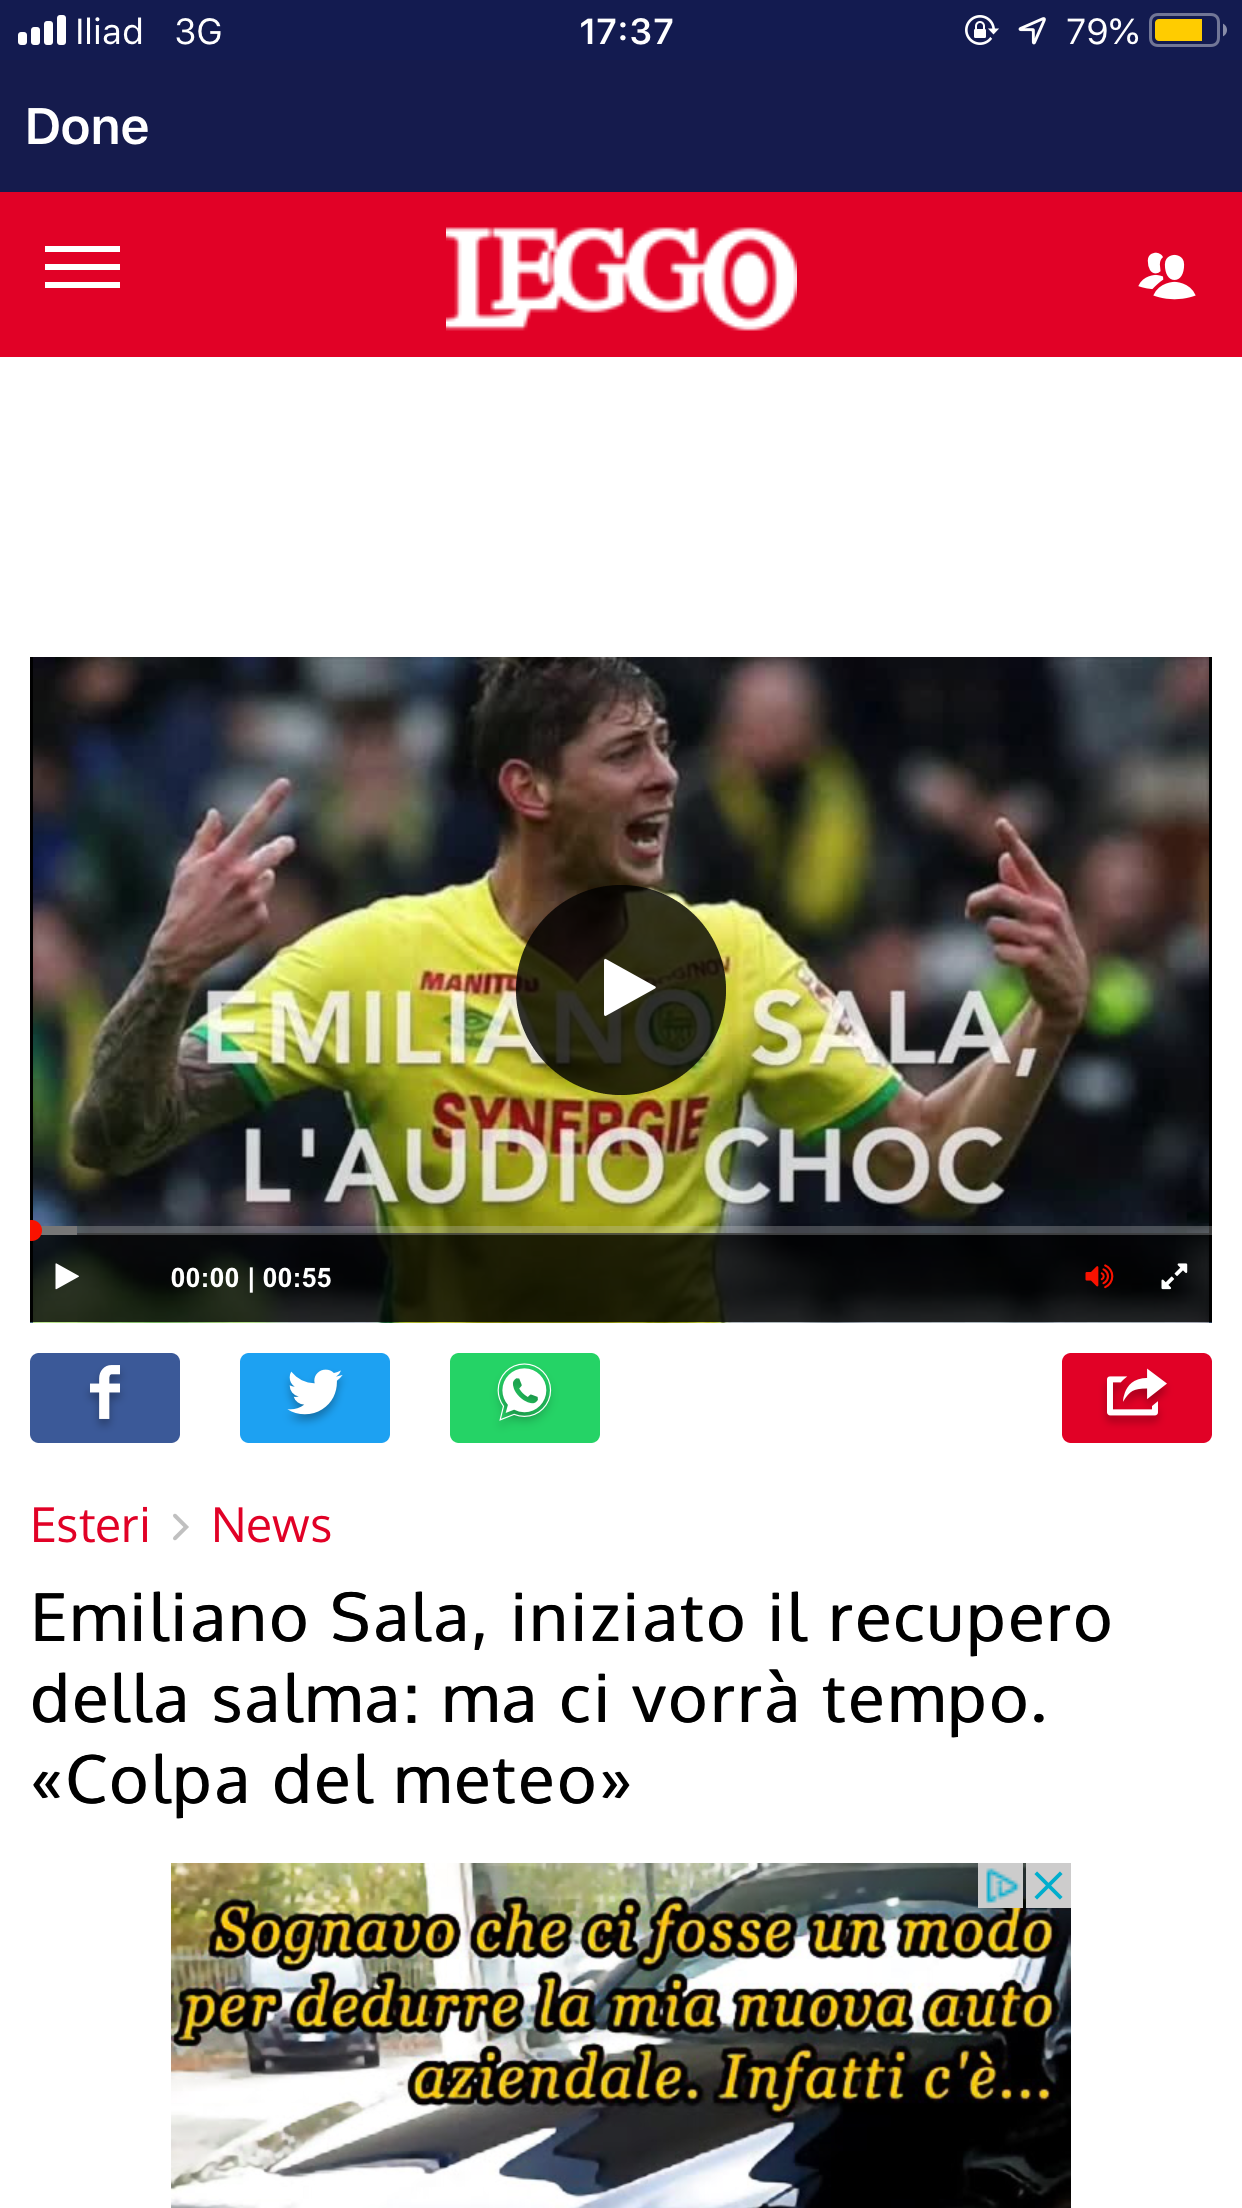
\includegraphics[width=.8\linewidth]{images/Screen/WebView}
		\caption{WebView to see and read the complete article from the origin website}
	\end{subfigure}
\end{figure}

\subsection*{Live}

\begin{figure}[H]
	\begin{subfigure}{.5\textwidth}
		\centering
		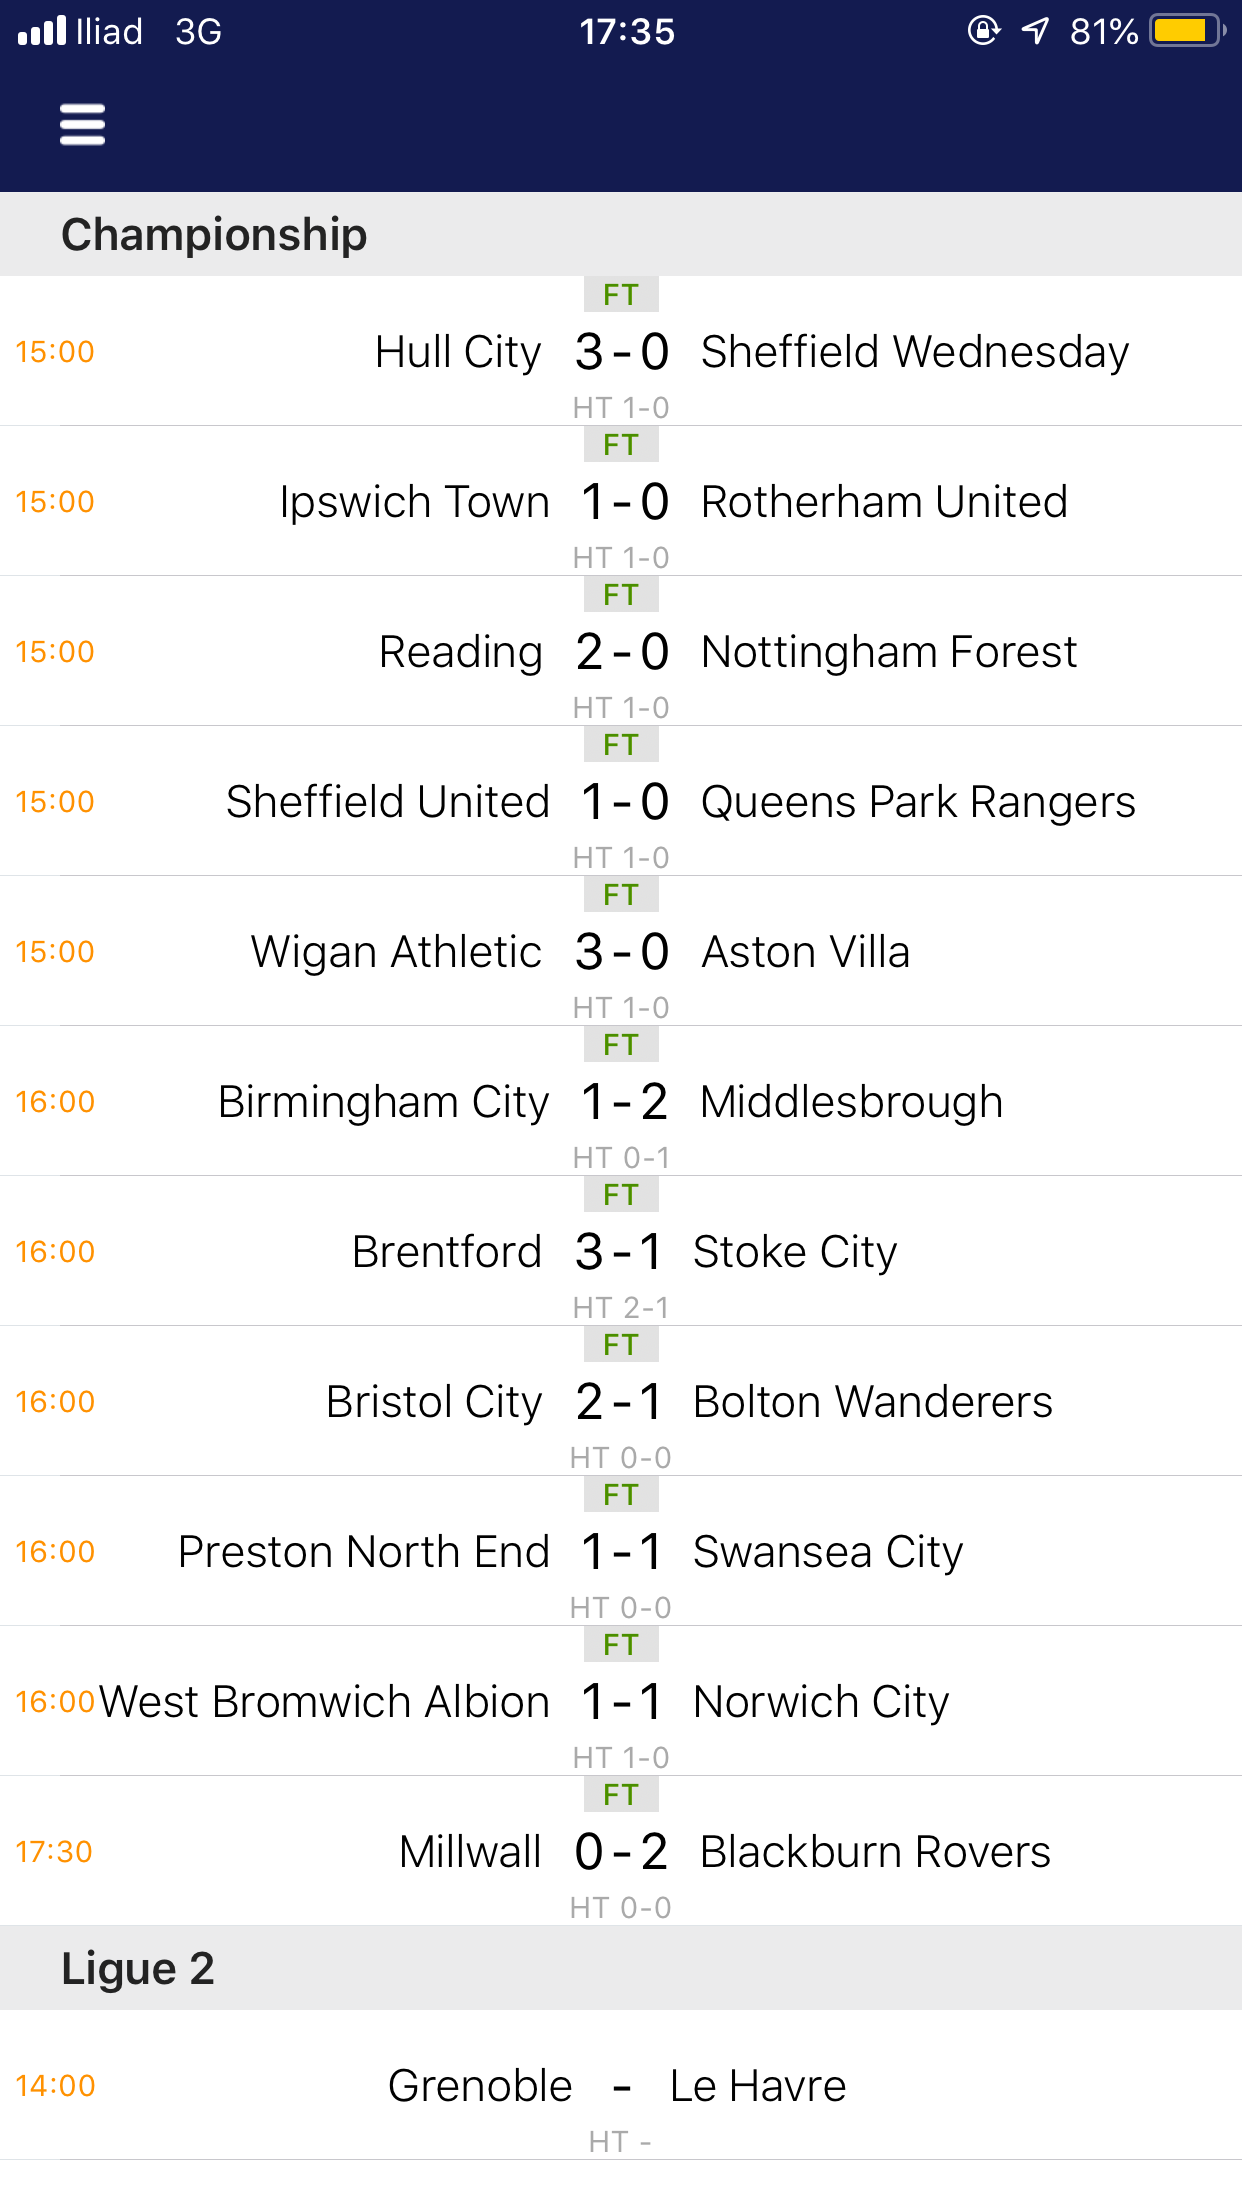
\includegraphics[width=.8\linewidth]{images/Screen/Live}
		\caption{This screen shows real time games}
	\end{subfigure}
	\begin{subfigure}{.5\textwidth}
		\centering
		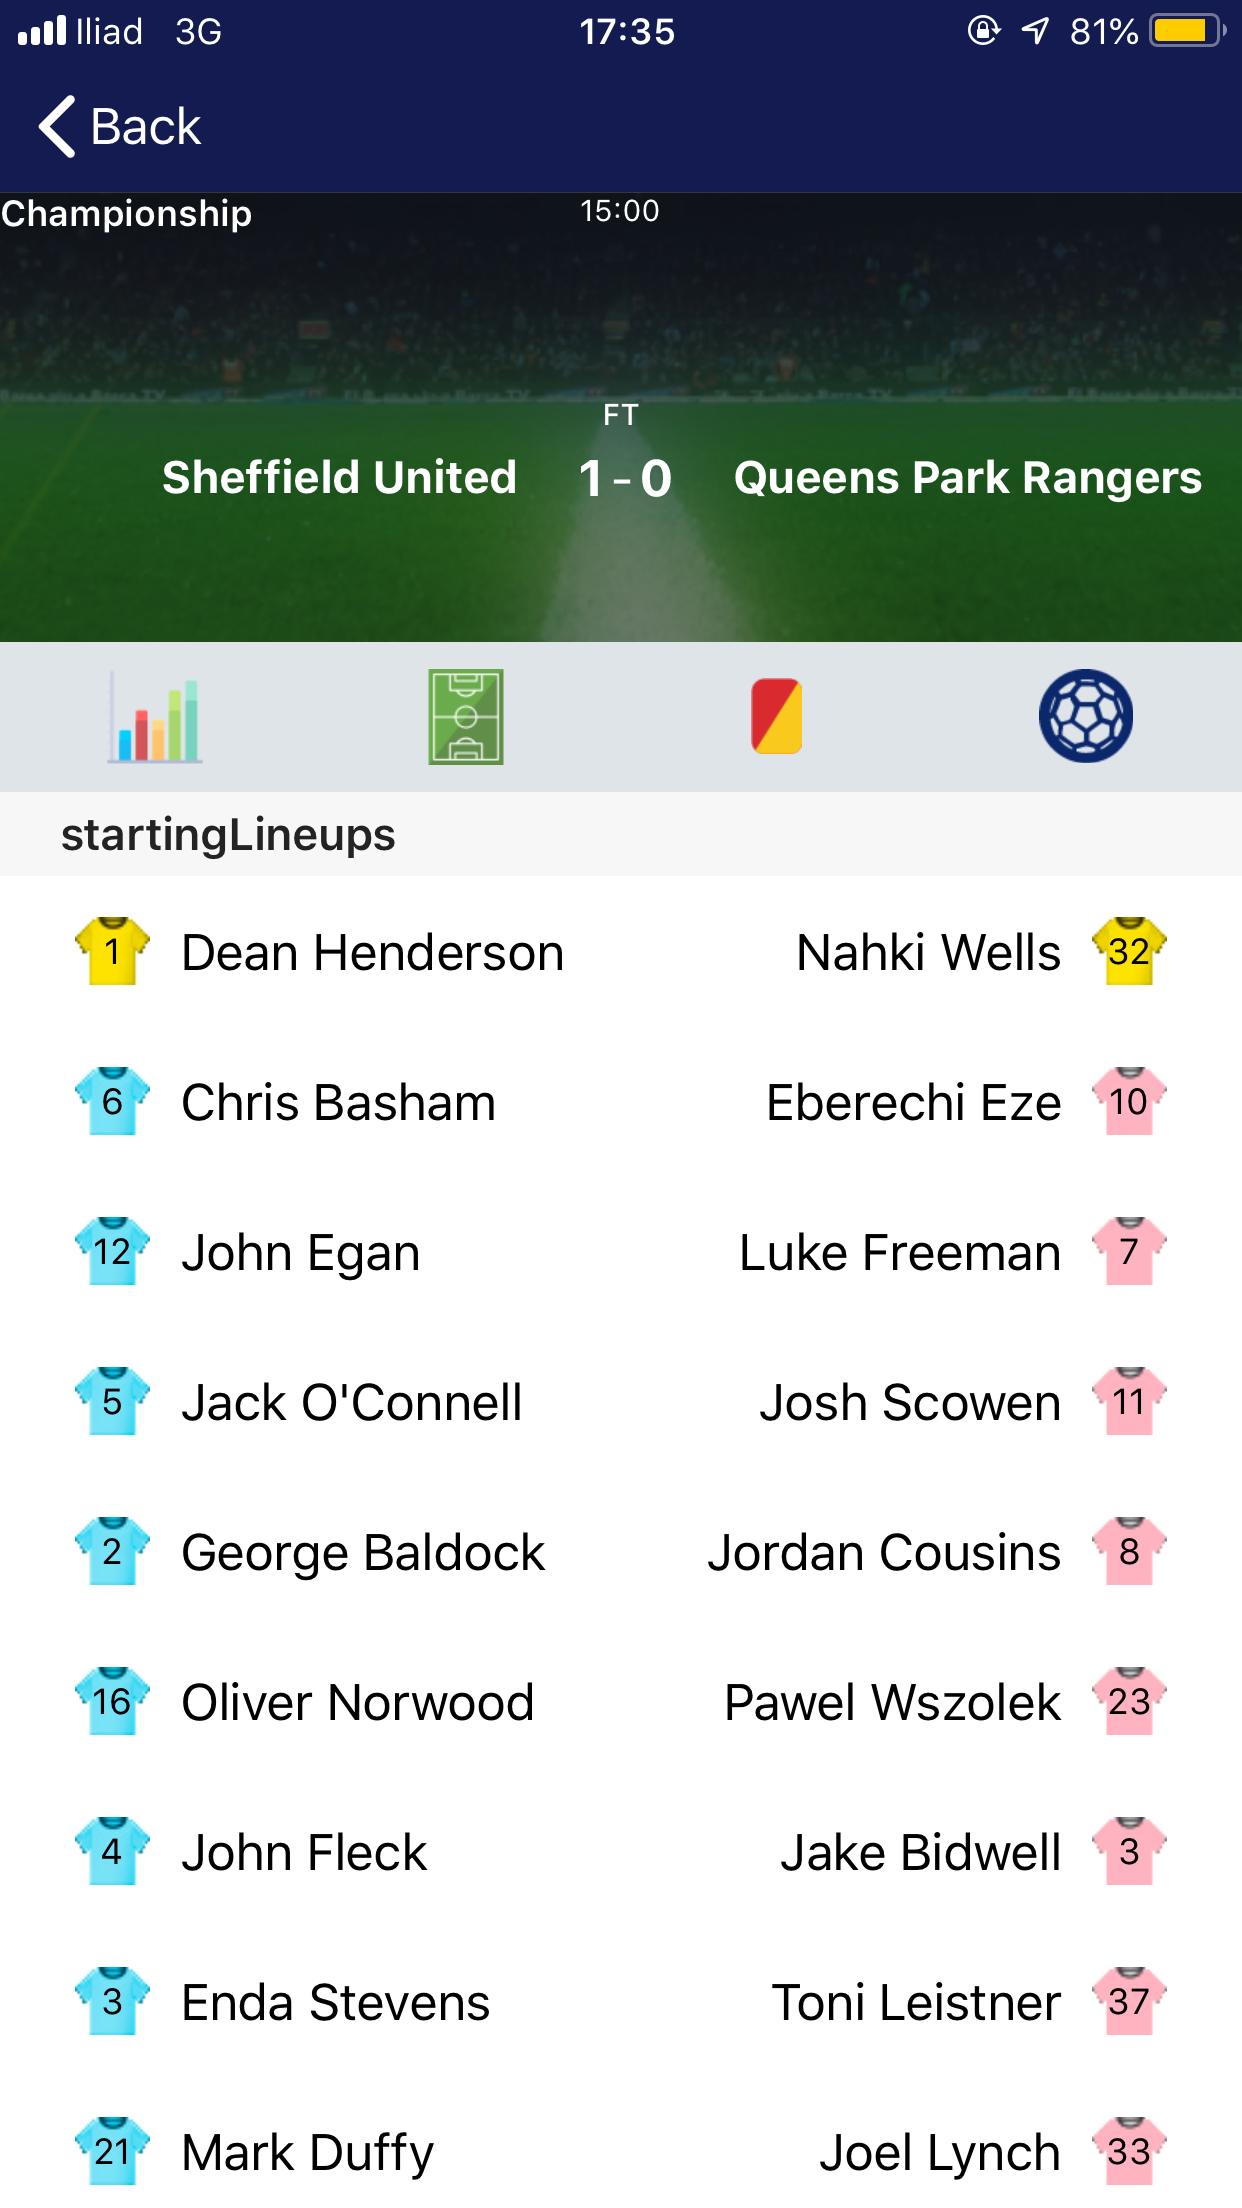
\includegraphics[width=.8\linewidth]{images/Screen/Formazione}
		\caption{In this screen are shown both teams lineups}
	\end{subfigure}
\end{figure}

\begin{figure}[H]
	\begin{subfigure}{.5\textwidth}
		\centering
		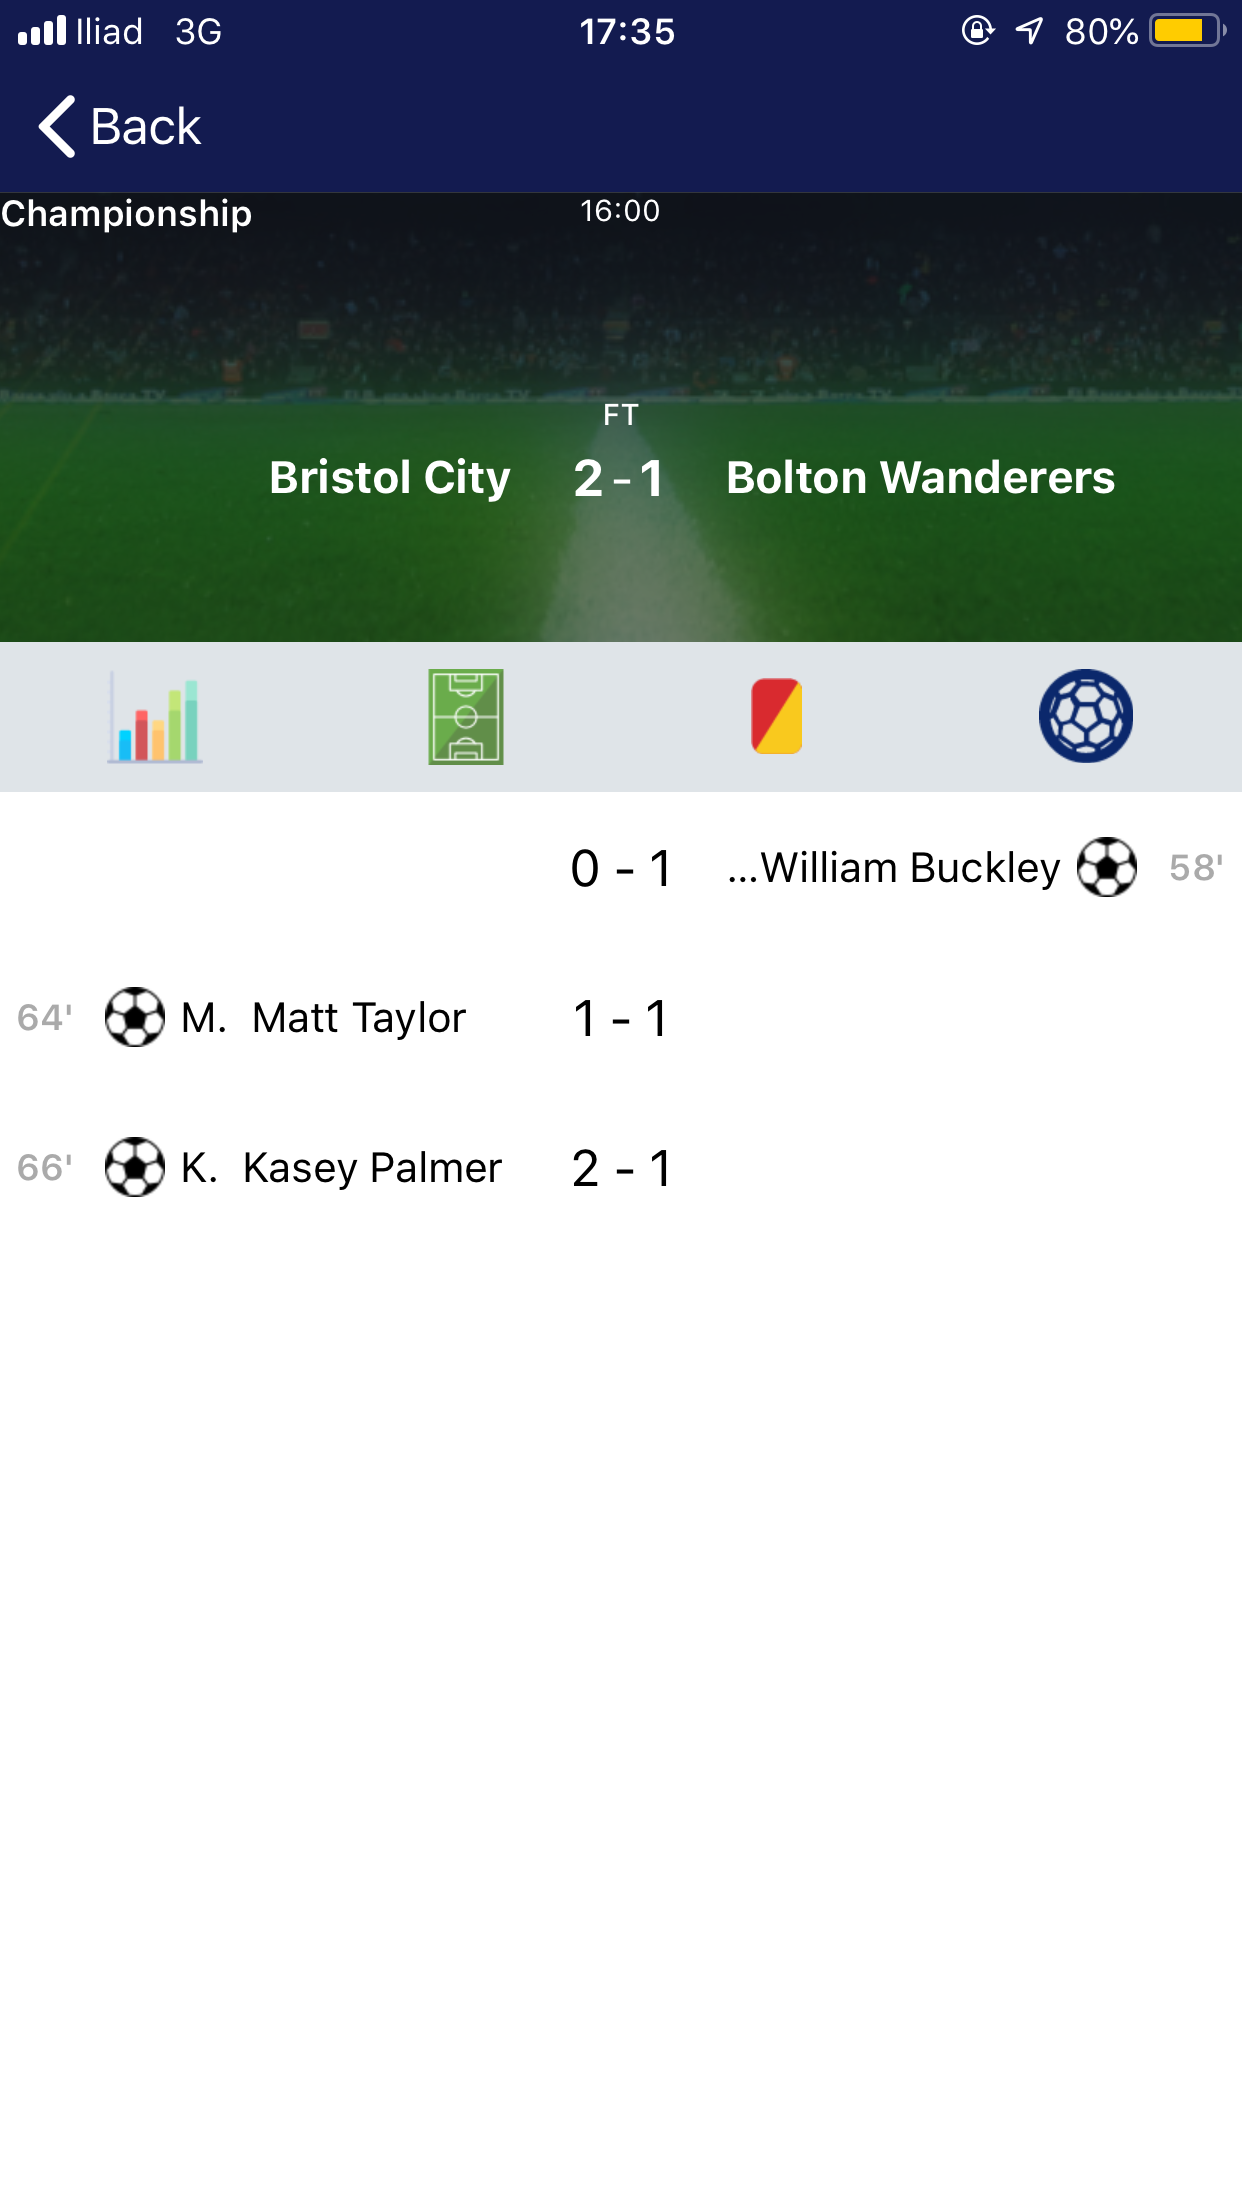
\includegraphics[width=.8\linewidth]{images/Screen/Goal}
		\caption{This screen shows the goals}
	\end{subfigure}
	\begin{subfigure}{.5\textwidth}
		\centering
		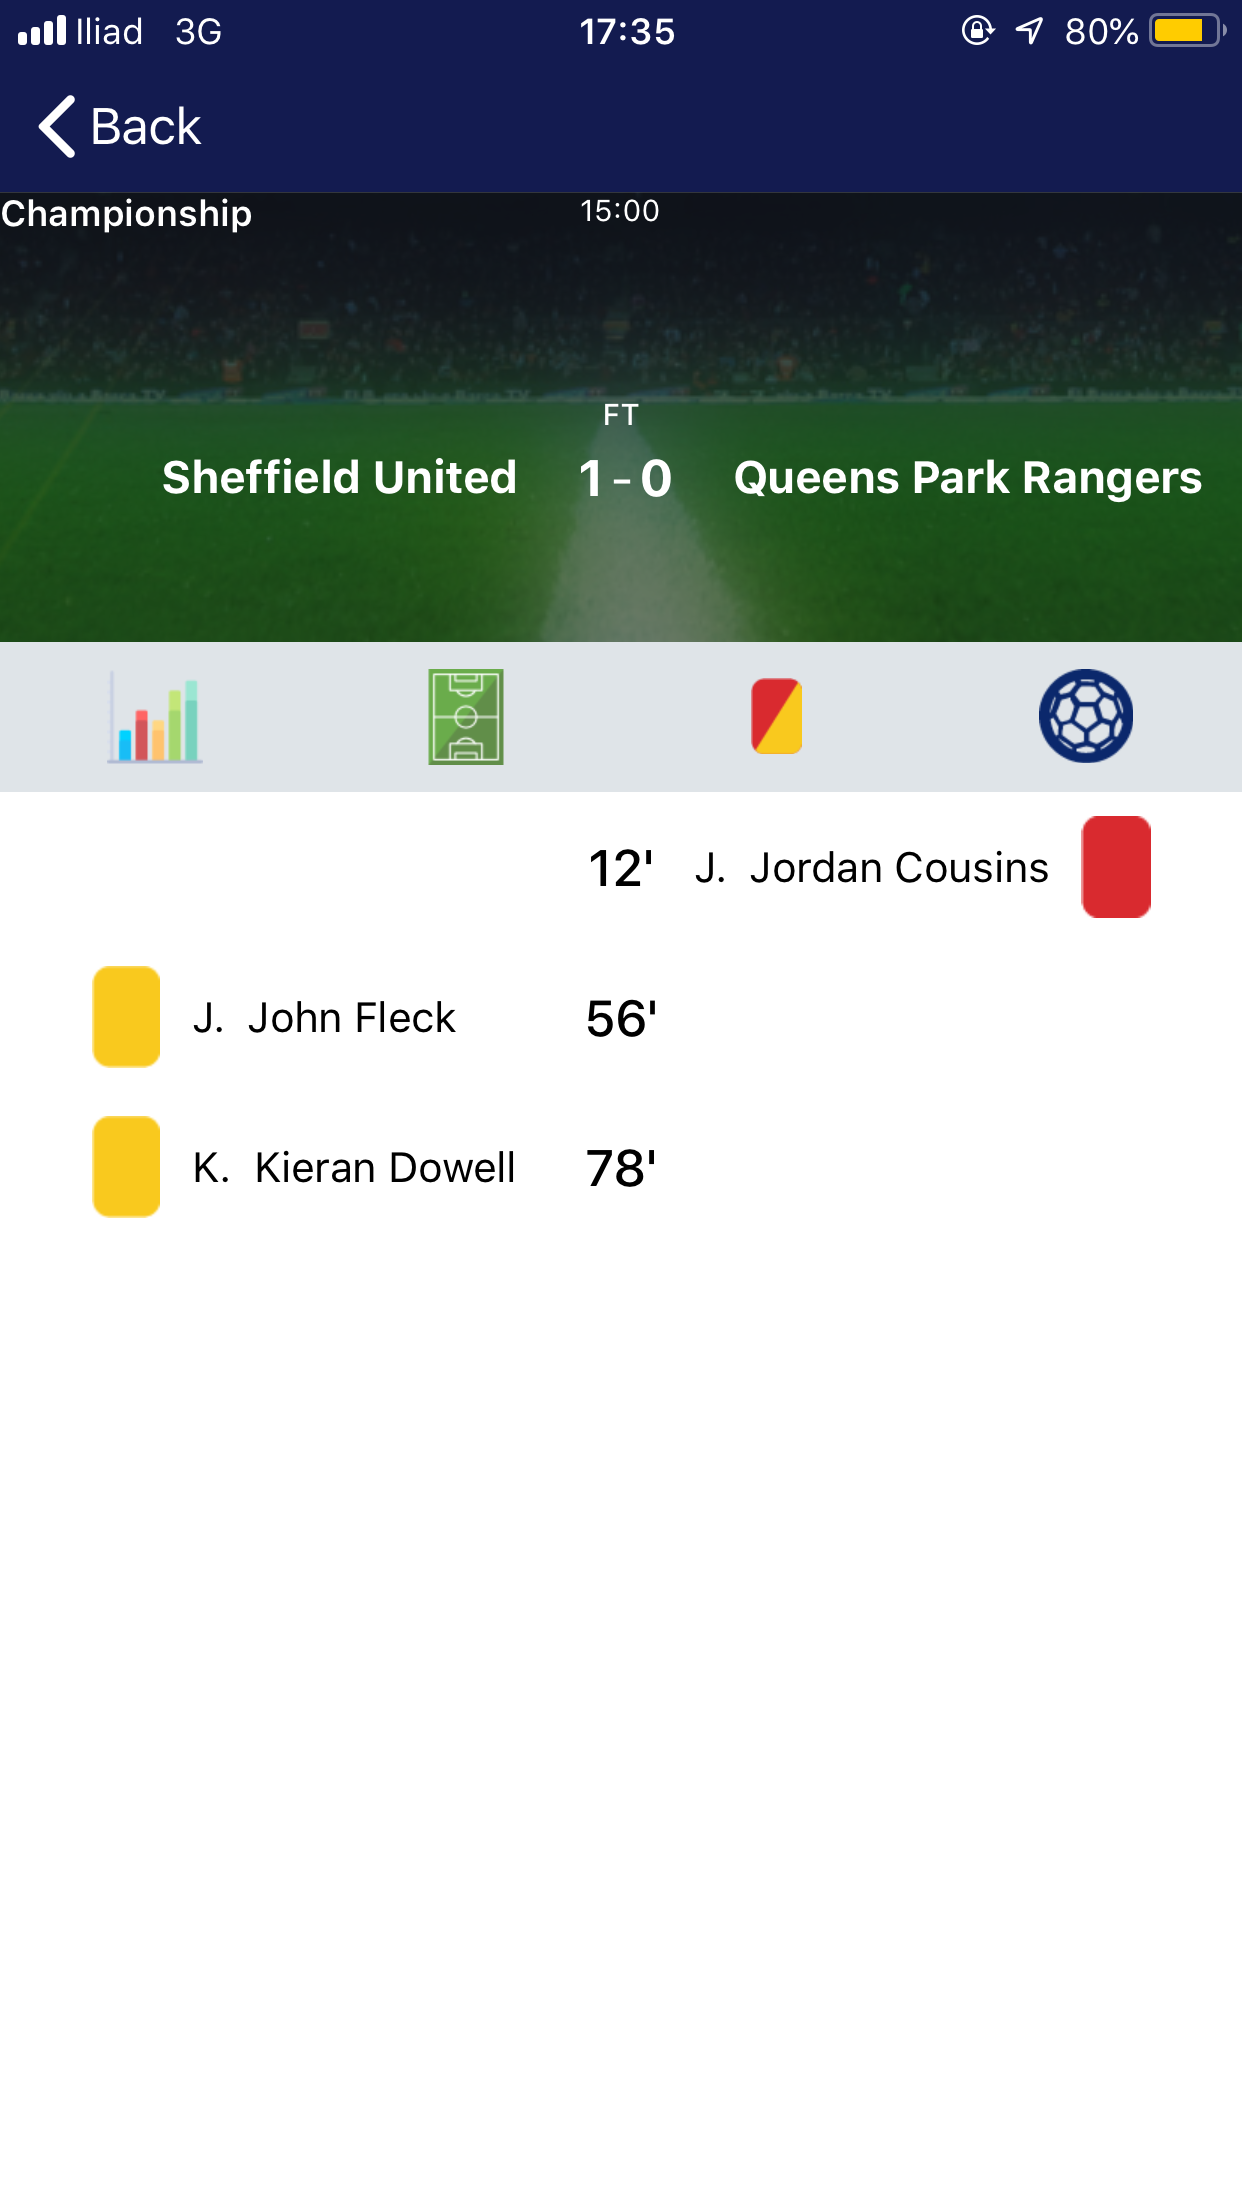
\includegraphics[width=.8\linewidth]{images/Screen/Cards}
		\caption{This screen shows the match cards}
	\end{subfigure}
\end{figure}

\begin{figure}[H]
	\centering
	\begin{subfigure}{.5\textwidth}
		\centering
		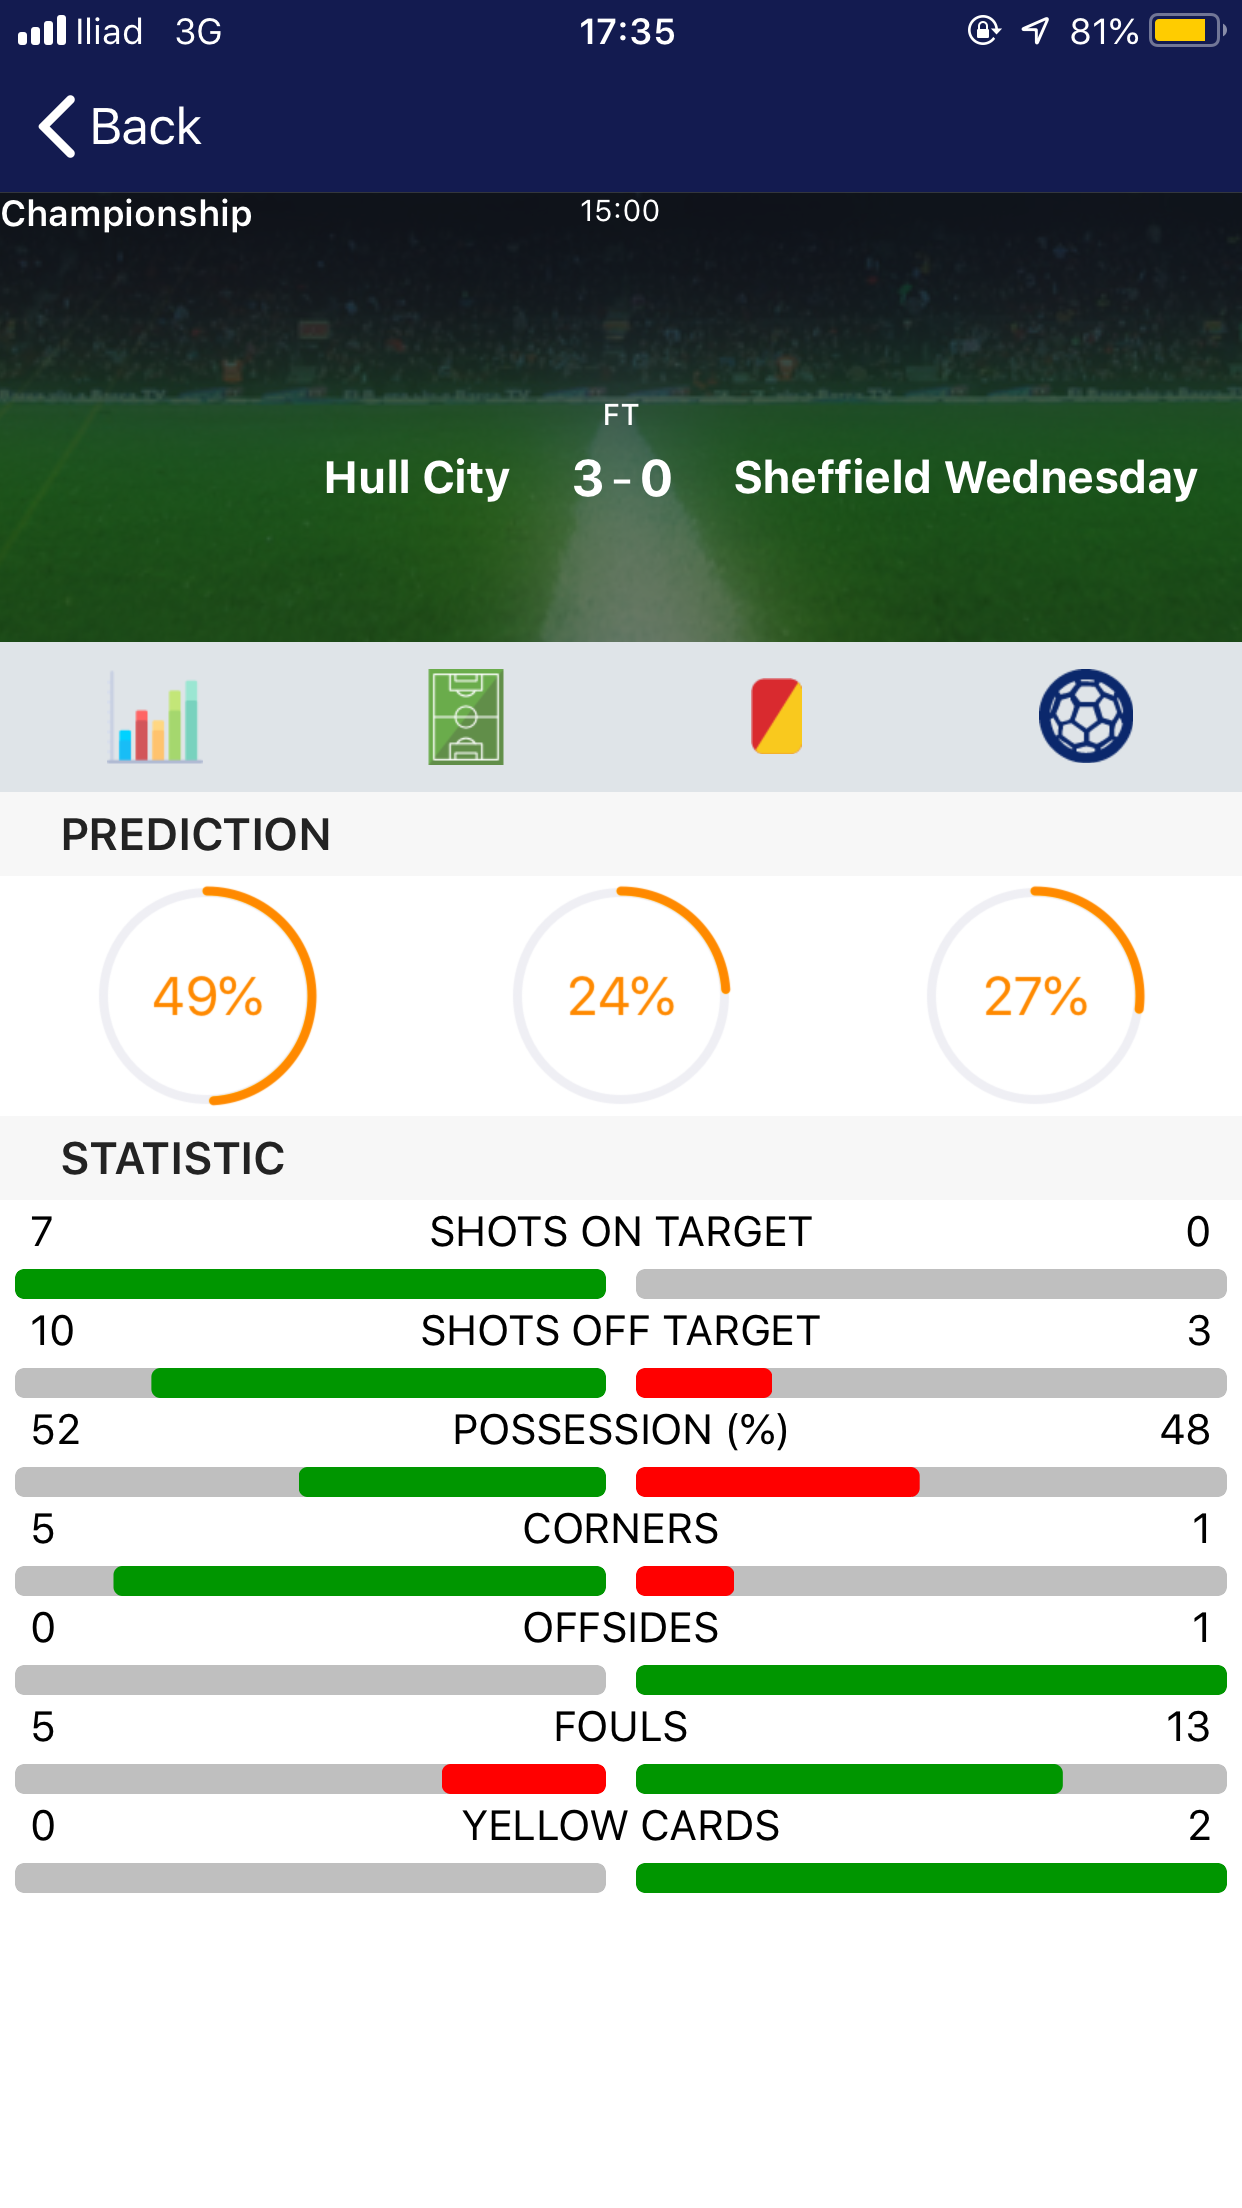
\includegraphics[width=.8\linewidth]{images/Screen/Statistica}
		\caption{This screen shows statistics}
	\end{subfigure}
\end{figure}

\subsection*{Odds}

\begin{figure}[H]
	\begin{subfigure}{.5\textwidth}
		\centering
		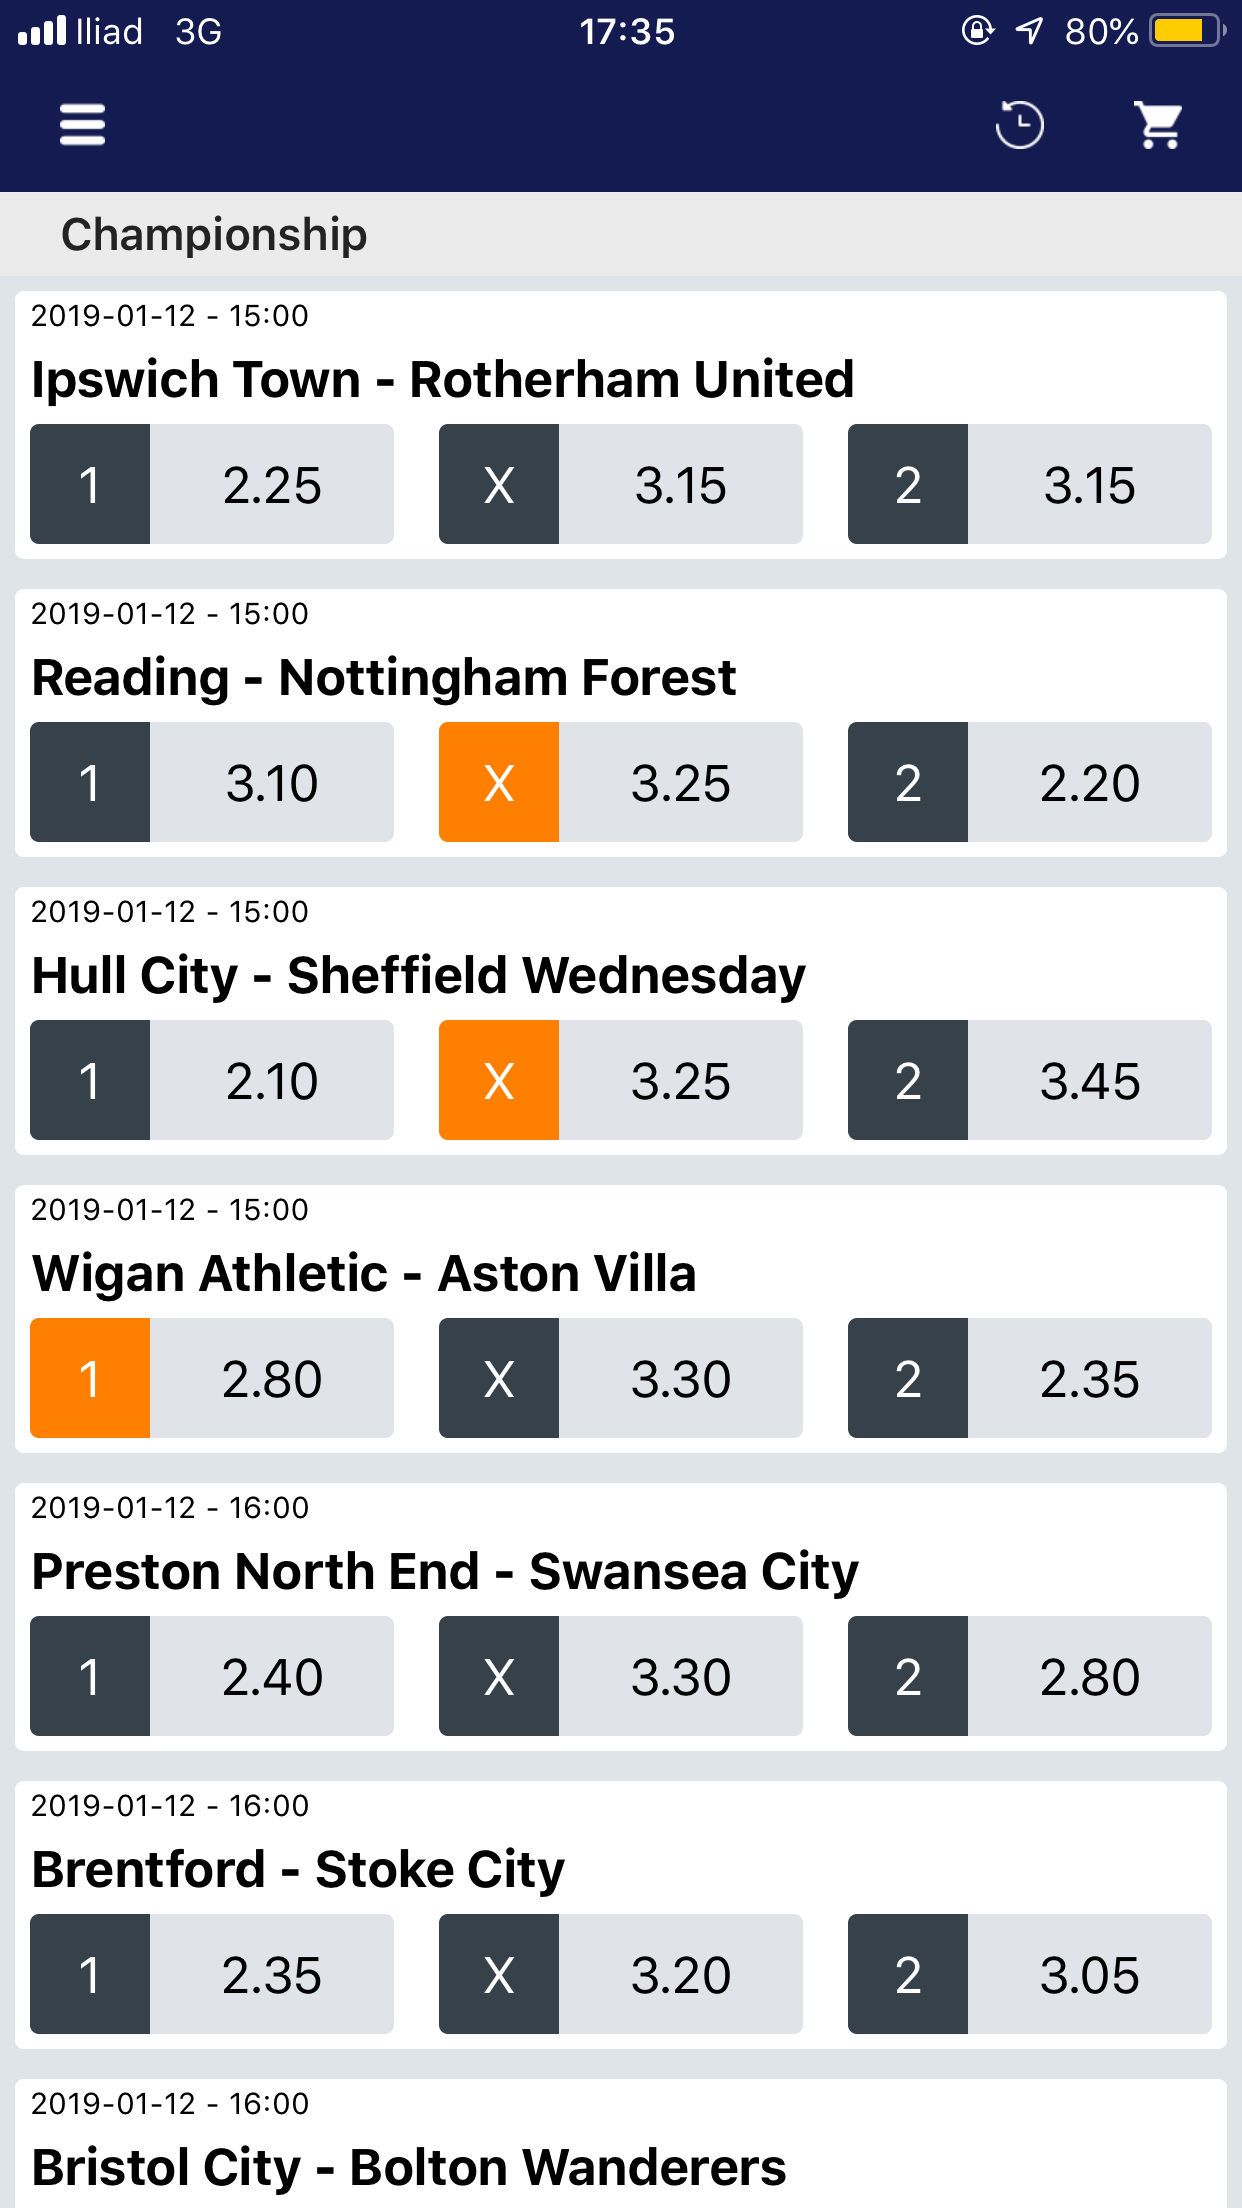
\includegraphics[width=.8\linewidth]{images/Screen/ComposizioneSchedina}
		\caption{This screen shows the act of composing a ticket}
	\end{subfigure}
	\begin{subfigure}{.5\textwidth}
		\centering
		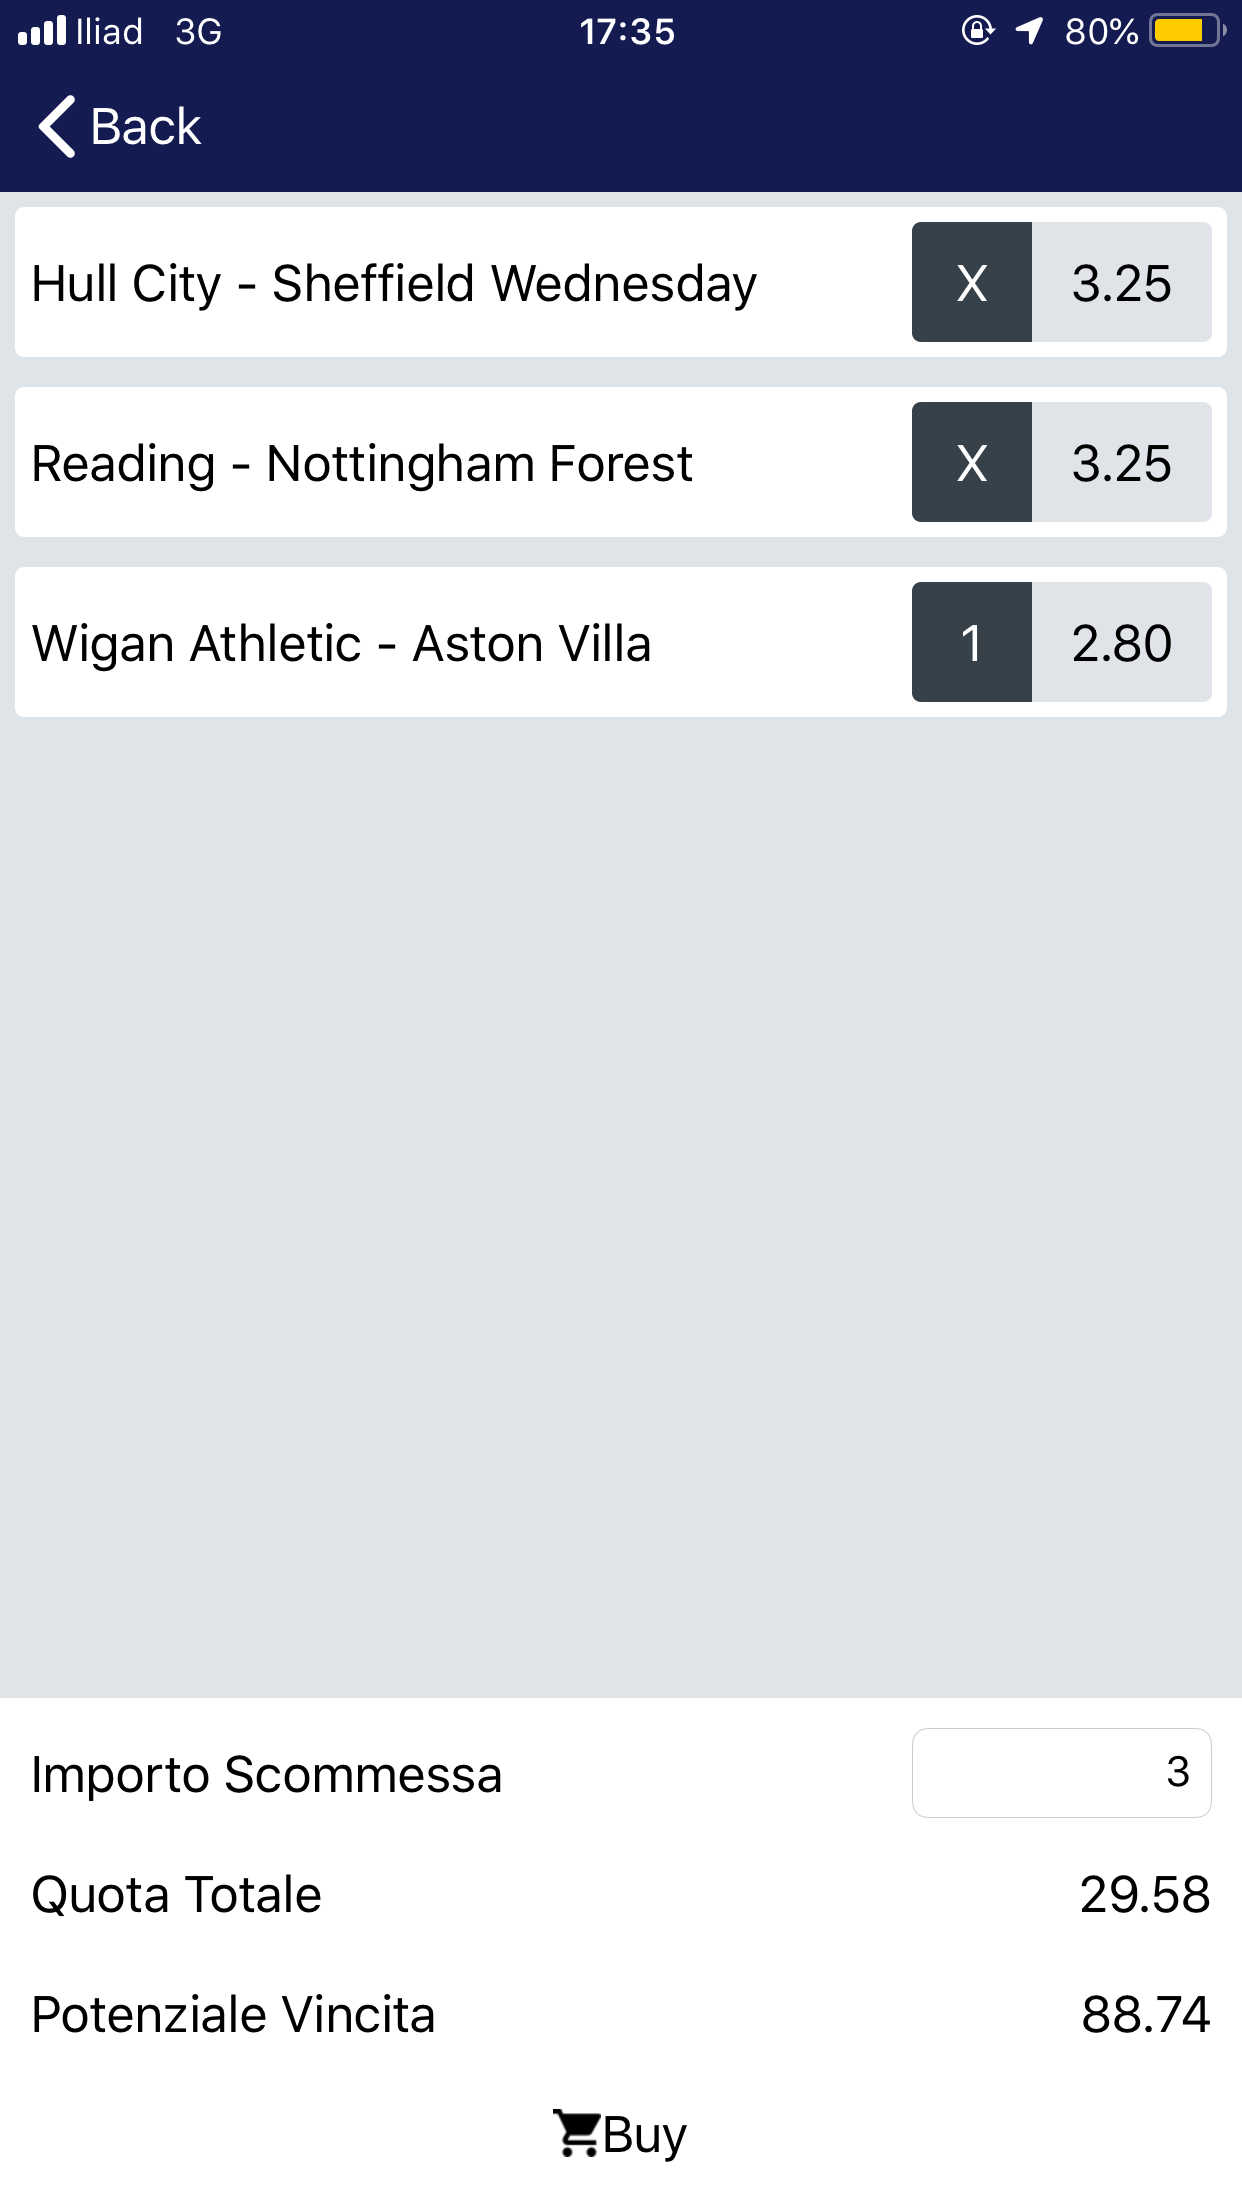
\includegraphics[width=.8\linewidth]{images/Screen/Carrello}
		\caption{This screen shows the bet}
	\end{subfigure}
\end{figure}


\begin{figure}[H]
	\centering
	\begin{subfigure}{.5\textwidth}
		\centering
		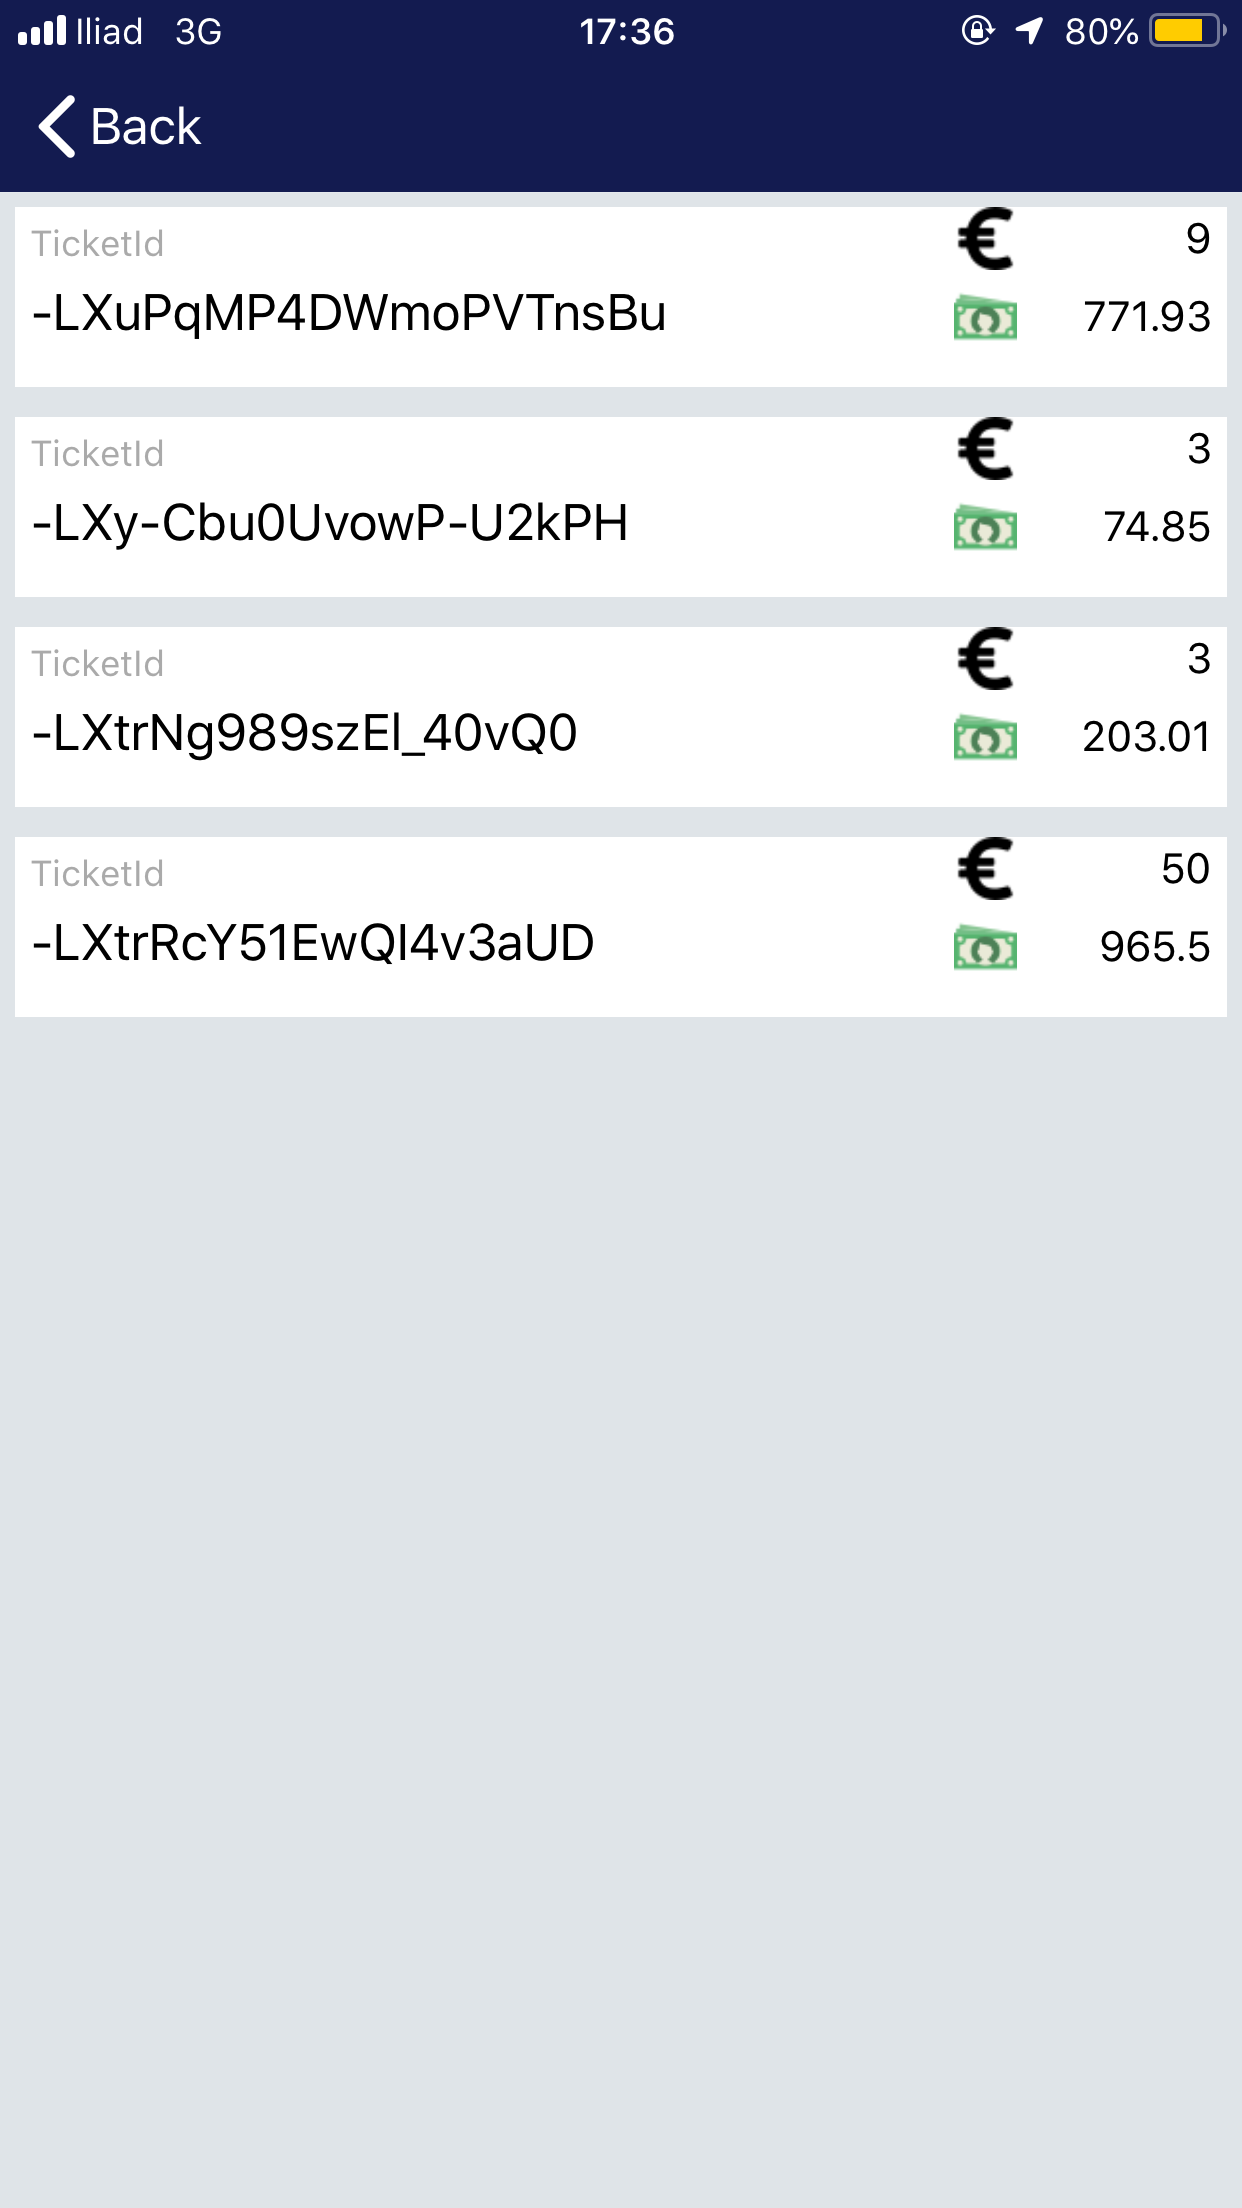
\includegraphics[width=.8\linewidth]{images/Screen/Storico}
		\caption{This screen shows the history of all the cards played}
	\end{subfigure}
\end{figure}

\subsection*{Chat}
\begin{figure}[H]
	\centering
	\begin{subfigure}{.5\textwidth}
		\centering
		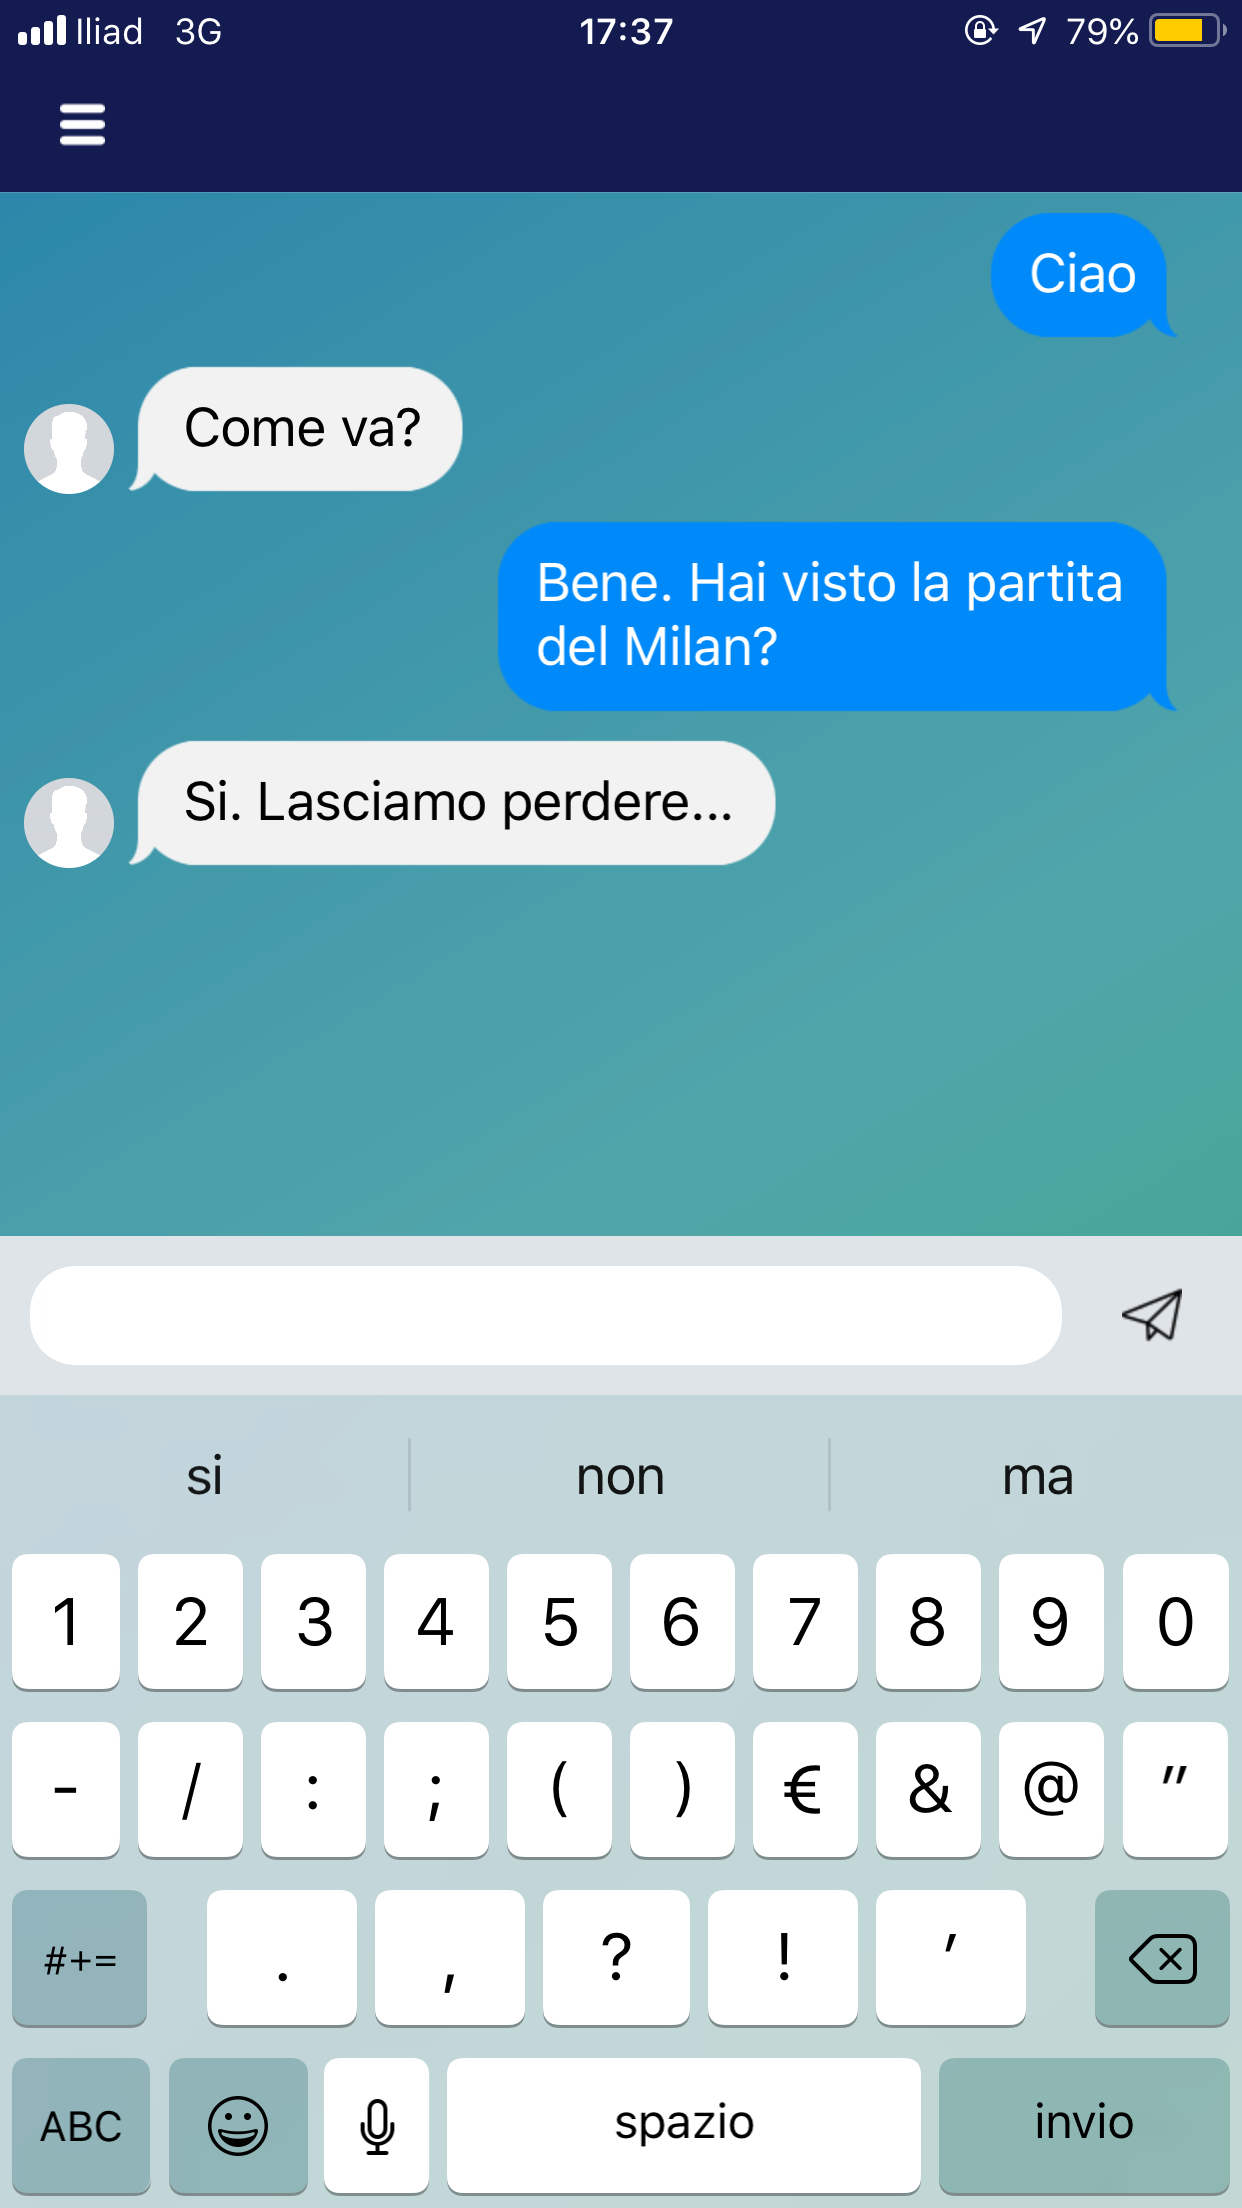
\includegraphics[width=.8\linewidth]{images/Screen/Chat}
		\caption{This screen shows the chat}
	\end{subfigure}
\end{figure}


\chapter{External Services and Libraries}
iSport application uses several third parties API in order to provide the user all the services.\\
The JSONDecoder component from UIKit was used to parse the JSON data.


\subsection*{Facebook SDK}
The Facebook SDK was used to manage the login. When a user wants to authenticate the application makes the call to the Facebook service through:
\begin{figure}[H]
	\centering
	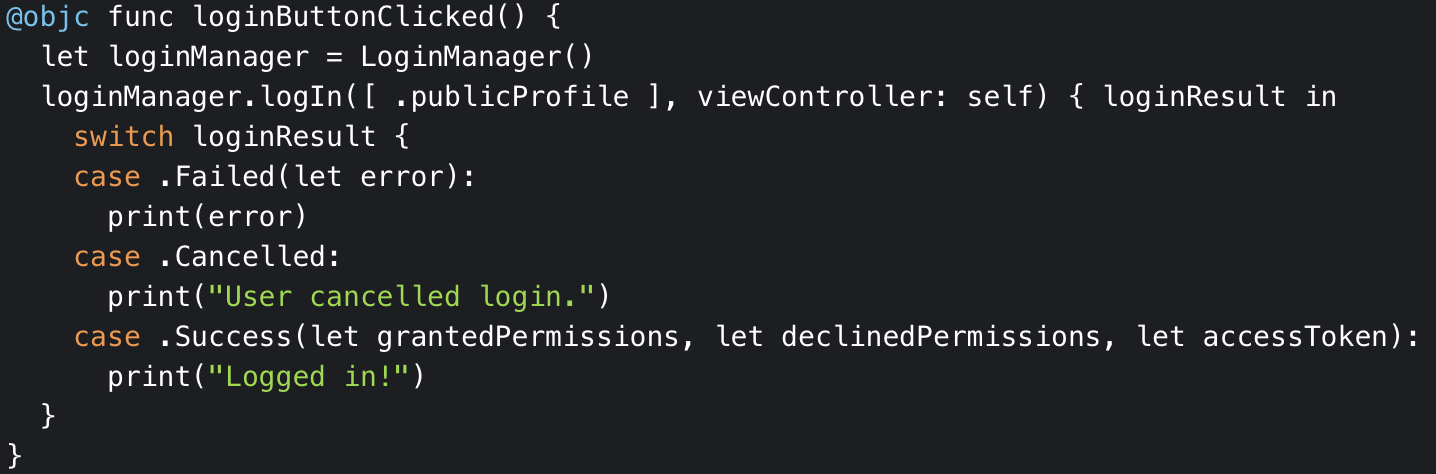
\includegraphics[width=0.7\textwidth]{images/LoginMethod}
\end{figure}
This method is used to send the user on Facebook for the authentication; once authenticated the user redirected to ”iSport” which will store the token provided.

Instead, the ”Graph API” is used for news publishing:
\begin{figure}[H]
	\centering
	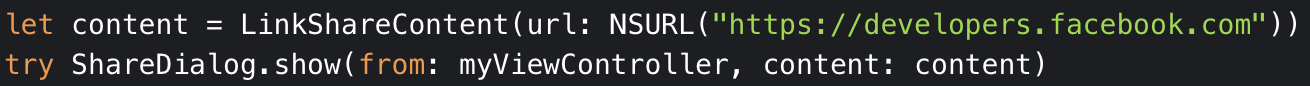
\includegraphics[width=0.7\textwidth]{images/GraphAPI}
\end{figure}

The following pods were included to use Facebook:
\begin{lstlisting}[style=CStyle]
pod 'FacebookCore'
pod 'FacebookLogin'
pod 'FacebookShare'
\end{lstlisting}

\subsection*{Firebase SDK}
Firebase SDKs are used to access the database. In particular, login is possible only inserting Facebook credentials in order to have a single login.

\begin{figure}[H]
	\centering
	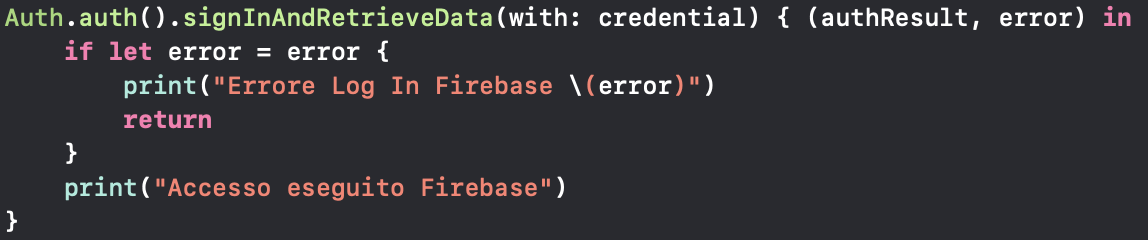
\includegraphics[width=0.7\textwidth]{images/LoginFirebase}
\end{figure}
For database access, the DatabaseManager included in the SDKs was used:
\begin{figure}[H]
	\centering
	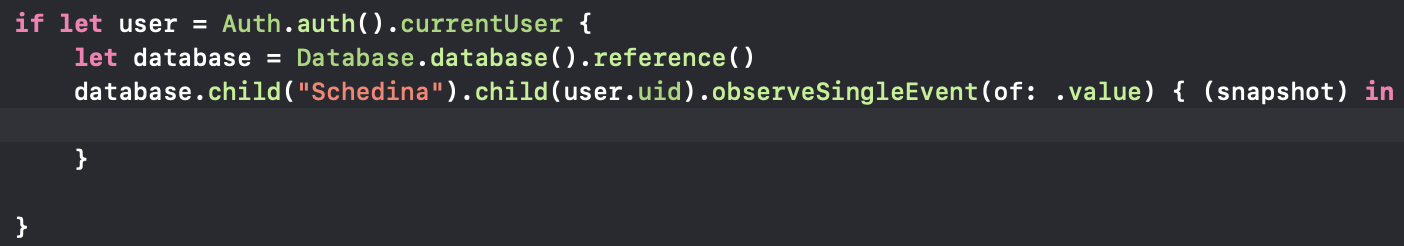
\includegraphics[width=0.7\textwidth]{images/DBaccess}
\end{figure}
The following pods were included to use Firebase:
\begin{lstlisting}[style=CStyle]
pod 'Firebase/Core'
pod 'Firebase/Auth'
pod 'Firebase/Database'
\end{lstlisting}

\subsection*{Scaledrone}
Scaledrone API was used for the real-time chat service. The following extension is used to connect to the room:
\begin{figure}[H]
	\centering
	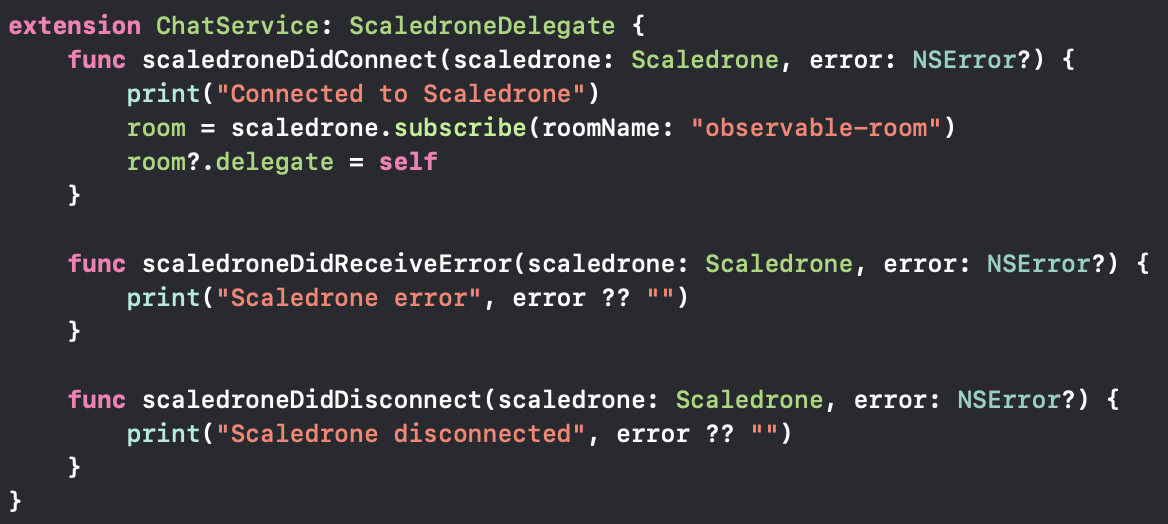
\includegraphics[width=0.7\textwidth]{images/ScaledroneConnect}
\end{figure}
While for receiving messages:
\begin{figure}[H]
	\centering
	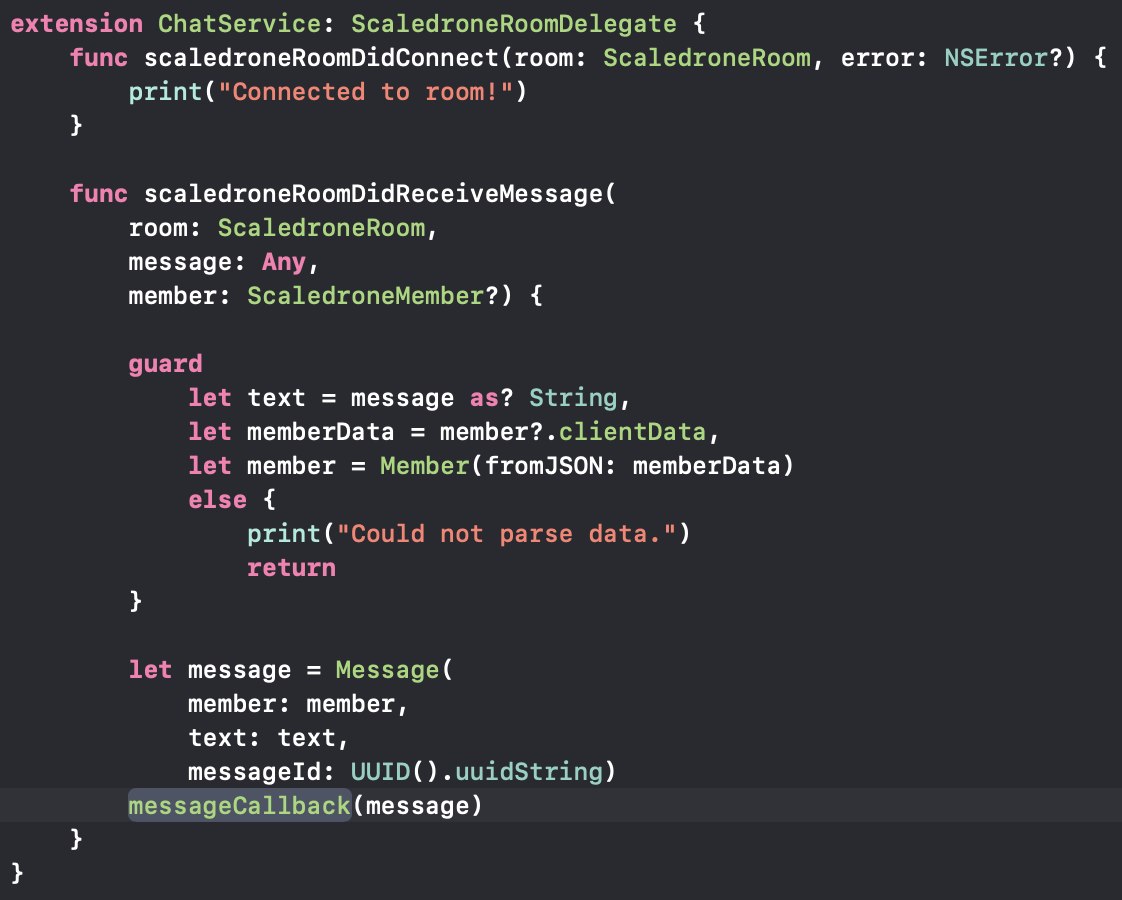
\includegraphics[width=0.7\textwidth]{images/ScaledroneReceive}
\end{figure}
The following pods were included to use the Scaledrone service:
\begin{lstlisting}[style=CStyle]
pod 'Scaledrone', '~> 0.3.0'
\end{lstlisting}

\subsection*{NewsAPI}
If a user wants to see the most important daily news, the application will perform the following operations:
\begin{itemize}
	\item sends a GET request to the endpoint supplied by the service
	\item If the answer is valid, it parses the JSON content
	\item Creates the table cells containing the information provided and parsed by the service 
	\item Download preview images asynchronously
\end{itemize}
The endpoint used is "https://newsapi.org/v2/top-headlines?country=it\&category=sports \&apiKey=API\_KEY". The answer provided by the service is:
\begin{figure}[H]
	\centering
	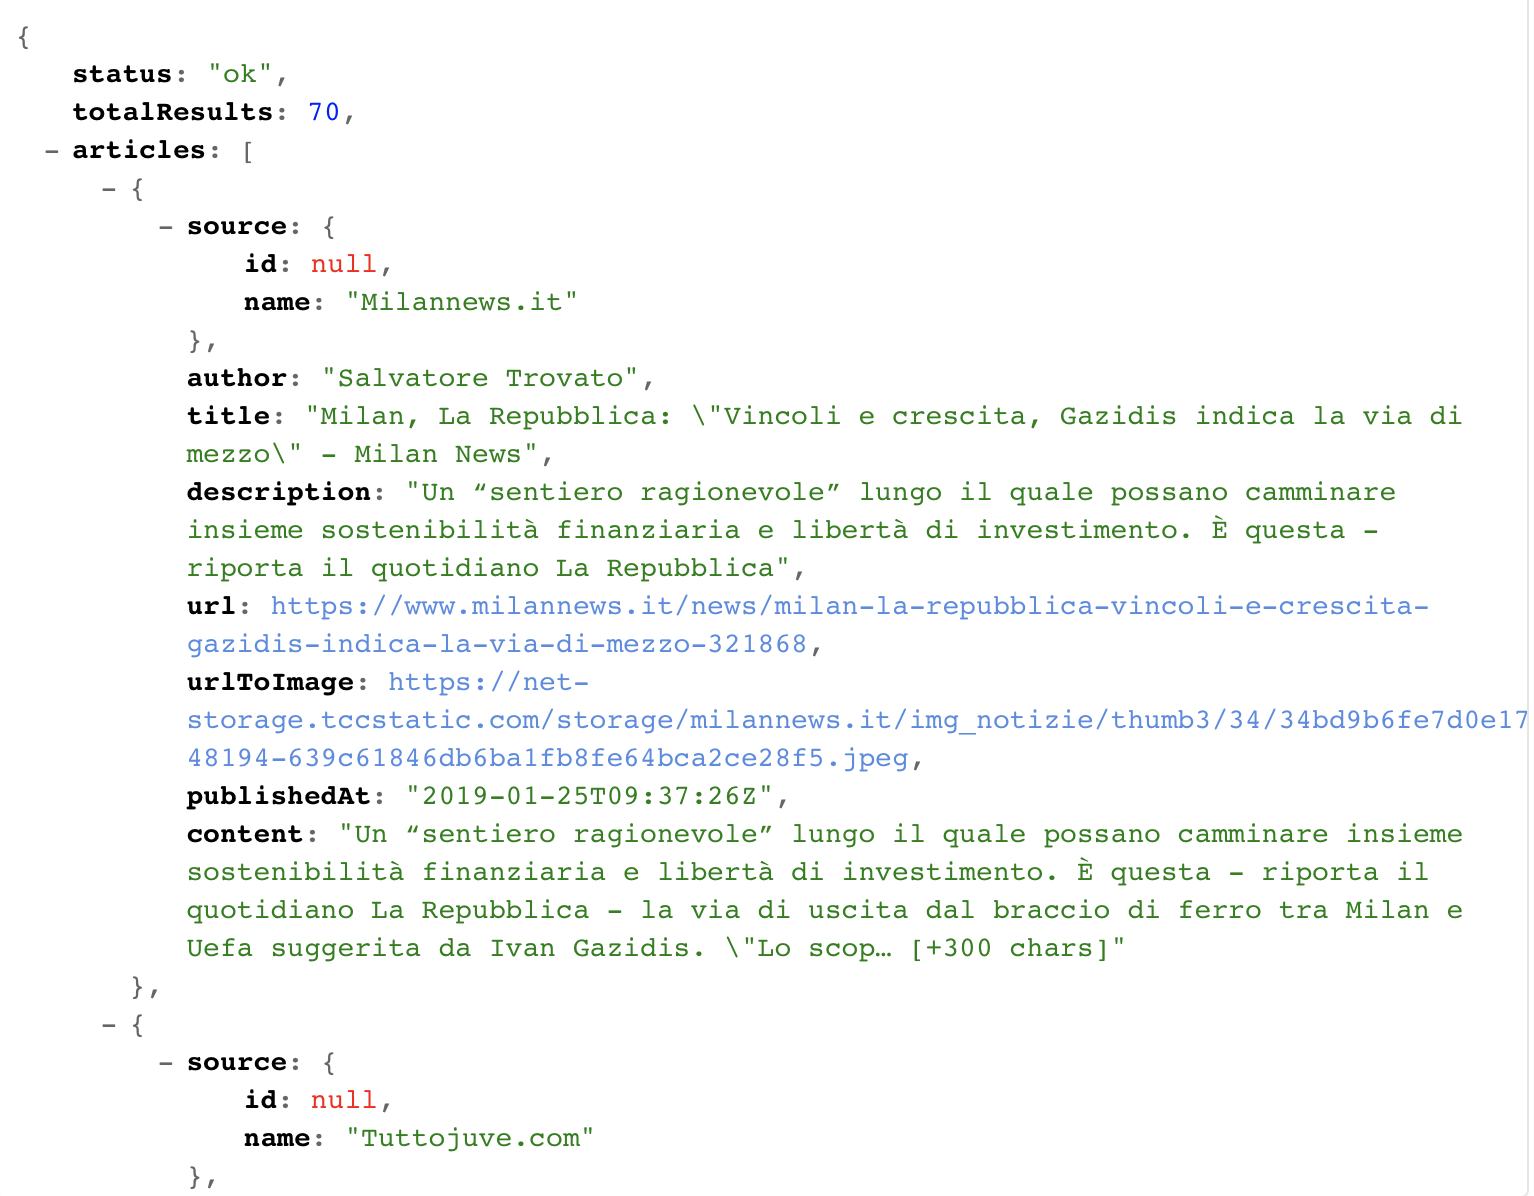
\includegraphics[width=0.7\textwidth]{images/ResponseNewsAPI}
\end{figure}
The following data structure was used for the parsing:
\begin{figure}[H]
	\centering
	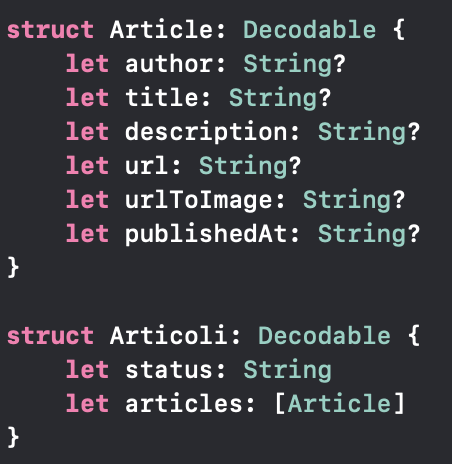
\includegraphics[width=0.3\textwidth]{images/StructDati}
\end{figure}
\subsection*{APIFootball}
When a user wants to see a daily match score the application performs the following operations:
\begin{itemize}
	\item sends a GET request to the endpoint supplied by the service
	\item If the answer is valid, it parses the JSON content
	\item Creates the table cells containing the information provided and parsed by the service 
	\item Update the information every 30 seconds
\end{itemize}
The endpoint used to obtain the results is "https://apifootball.com/api/?action=get\_events". The answer provided by the service is:
\begin{figure}[H]
	\centering
	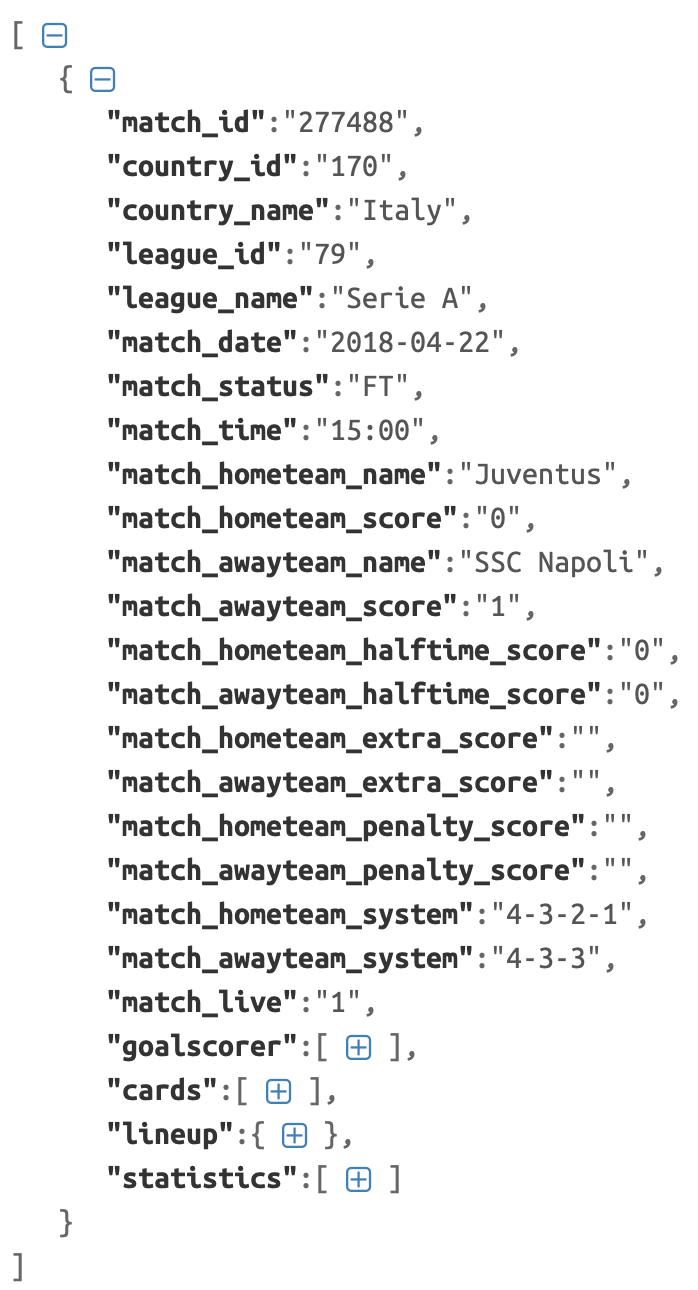
\includegraphics[width=0.3\textwidth]{images/ResponseCompleta}
\end{figure}
The following data structure was used for the parsing:
\begin{figure}[H]
	\centering
	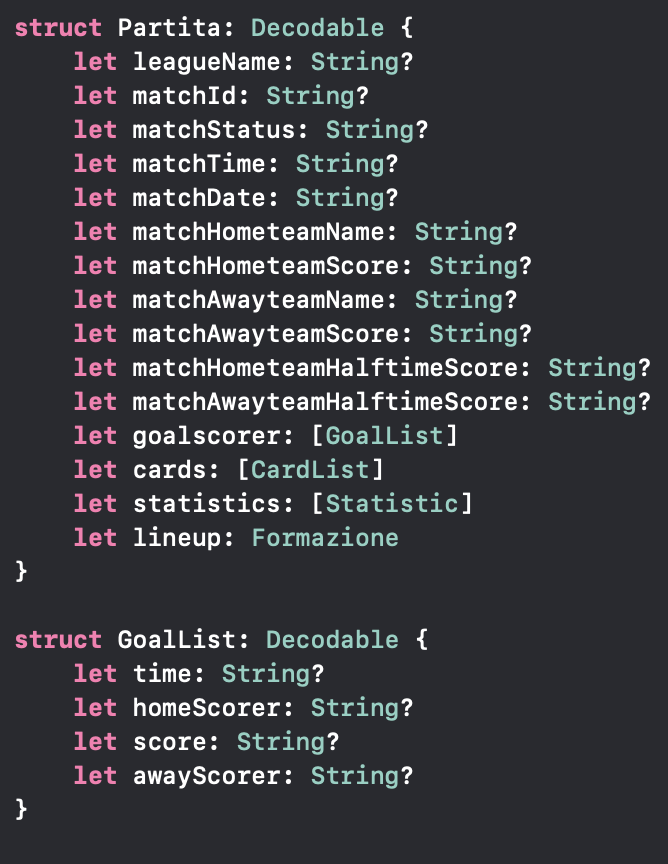
\includegraphics[width=0.3\textwidth]{images/StructPartita2}
	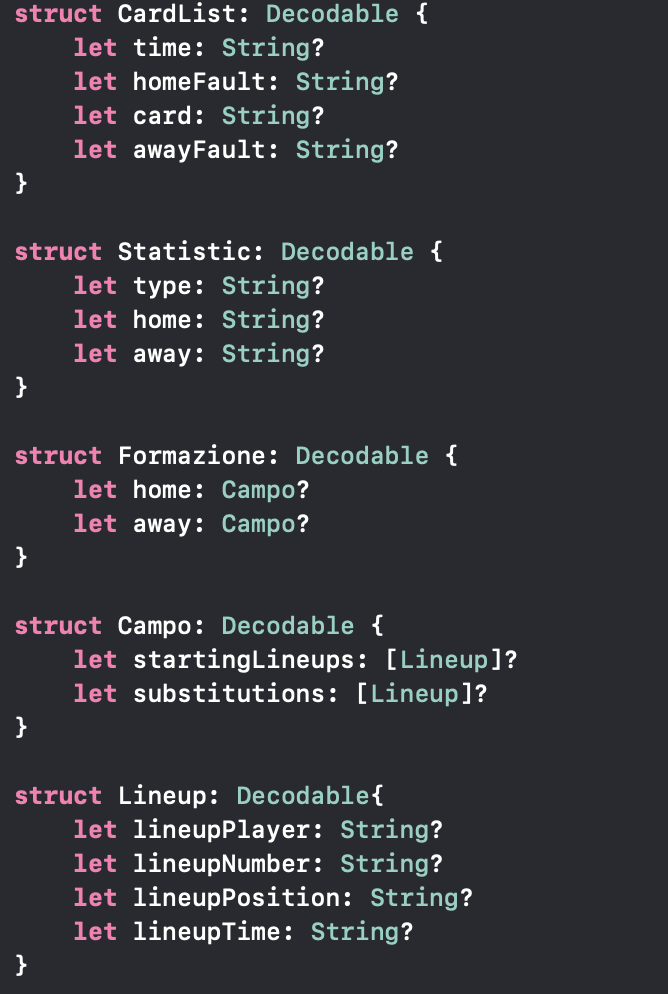
\includegraphics[width=0.3\textwidth]{images/StructPartita1}
\end{figure}
To get the game’s predictions, the endpoint used is "https://apifootball.com/api/? action=get\_predictions". The answer provided by the service is:
\begin{figure}[H]
	\centering
	\includegraphics[width=0.3\textwidth]{images/ResponsePrediction}
\end{figure}
The following data structure was used for the parsing:
\begin{figure}[H]
	\centering
	\includegraphics[width=0.3\textwidth]{images/StructPrediction}
\end{figure}
To get the odds of the games the endpoint used is "https://apifootball.com/api/? action=get\_odds". The answer provided by the service is:
\begin{figure}[H]
	\centering
	\includegraphics[width=0.3\textwidth]{images/ResponseOdds}
\end{figure}
The following data structure was used for the parsing:
\begin{figure}[H]
	\centering
	\includegraphics[width=0.3\textwidth]{images/StructOdds}
\end{figure}


\chapter{Software System Attribute}
\section{Reliability}
As the majority of function requires an internet connection, the software is reliable as long as there are no connectivity problems.
\section{Availability}
The availability parameter also relies on the internet connection signal and on the responses provided by "https://newsapi.org" and "https://apifootball.com". No problems of availability were found both during the developement phase and beta testing with users.
\section{Security}
The security of the iSport application was the main concern during the developement. As all the information provided are retrived from the web, there are different checks to perform in order to keep the user information safe. Furthermore, for the communication with external services, was chosen HTTPS protocol to guarantee greater security
\section{Maintainability}
The entire application is very maintainable as the code is entirely documented, in particular in several critical function. Therefore any developer who wants to improve it or make changes is able to do it without relevant difficulty.
\section{Usability}
The usability was another of our concern for the development. In order to improve it, a beta version of the application was given to 5 users and tested for 1 weeks. The result of this test highlighted usability issues. In particular, in the first version the buttons for changing information on the match detail page were not clearly visible. Another report concerned the lack of visual feedback after adding a quota to their ticket. Both of these problems were then solved in a later version of the application.

\chapter{Test Cases}
As the structure of our application is mainly based on creating elemnents on screen starting from data received from the web, a unit test for each asynchronous function was not a viable solution.\\

To test the app we used XCTest that is an Apple framework; it allows to analyze the execution flow through actions on UI, such as button tap. Moreover for some methods we used the Unit Test, for example calculation of the potential winning or JSON parse.\\

Below the results of the test execution:
\begin{figure}[H]
	\centering
	\includegraphics[width=0.8\textwidth]{images/TestUnit}
\end{figure}
\chapter{Tool \& Software Used}
For the developement the following tools and software were used:
\begin{itemize}
	\item Xcode 10.1
	\item GIMP
	\item Sketch
	\item Postman
	\item Draw.io
	\item Github
\end{itemize}






\end{document}
